\documentclass[review]{elsarticle}

\usepackage{lineno,hyperref}
\usepackage{eurosym}
\usepackage{rotating} 
\usepackage{times}
\usepackage{graphicx}
\usepackage{setspace}
\usepackage{amsmath}
\usepackage{epstopdf}
\usepackage[obeyFinal]{easy-todo}

\modulolinenumbers[5]

\journal{Journal of \LaTeX\ Templates}

%%%%%%%%%%%%%%%%%%%%%%%
%% Elsevier bibliography styles
%%%%%%%%%%%%%%%%%%%%%%%
%% To change the style, put a % in front of the second line of the current style and
%% remove the % from the second line of the style you would like to use.
%%%%%%%%%%%%%%%%%%%%%%%

%% Numbered
%\bibliographystyle{model1-num-names}

%% Numbered without titles
%\bibliographystyle{model1a-num-names}

%% Harvard
%\bibliographystyle{model2-names.bst}\biboptions{authoryear}

%% Vancouver numbered
%\usepackage{numcompress}\bibliographystyle{model3-num-names}

%% Vancouver name/year
%\usepackage{numcompress}\bibliographystyle{model4-names}\biboptions{authoryear}

%% APA style
%\bibliographystyle{model5-names}\biboptions{authoryear}

%% AMA style
%\usepackage{numcompress}\bibliographystyle{model6-num-names}

%% `Elsevier LaTeX' style
\bibliographystyle{elsarticle-num}
%%%%%%%%%%%%%%%%%%%%%%%


\begin{document}

\begin{frontmatter}

\title{Atomistic resolution structure and dynamics of lipid bilayers in simulations and experiments}
%\tnotetext[mytitlenote]{Fully documented templates are available in the elsarticle package on \href{http://www.ctan.org/tex-archive/macros/latex/contrib/elsarticle}{CTAN}.}

%% Group authors per affiliation:
%\author{O. H. Samuli Ollila \fnref{myfootnote}}
%\address{Radarweg 29, Amsterdam}
%\fntext[myfootnote]{Since 1880.}

%% or include affiliations in footnotes:
\author[mymainaddress]{O. H. Samuli Ollila\corref{mycorrespondingauthor}}
\cortext[mycorrespondingauthor]{Corresponding author}
\ead{samuli.ollila@aalto.fi}

\author[georgmainaddress,georgsecondaryaddress]{Georg Pabst}


\address[mymainaddress]{Department of Neuroscience and Biomedical Engineering, Aalto University}
\address[georgmainaddress]{University of Graz, Institute of Molecular Biosciences, Biophysics Division, NAWI Graz, Humboldtstr. 50/III, Graz, Austria}
\address[georgsecondaryaddress]{BioTechMed-Graz, Graz, Austria}


\begin{abstract}
Accurate details on the sampled atomistic resolution structures of lipid bilayers can be experimentally
obtained by measuring C--H bond order parameters, spin relaxation rates and scattering form factors.
These parameters can be also directly calculated from the classical atomistics resolution molecular dynamics
simulations (MD) and compared to the experimentally achieved results. This comparison measures
the simulation model quality with respect to `reality'. If agreement is sufficient, the simulation model
gives an atomistic structural interpretation of the aquired experimental data. Significant advance of MD 
models is made by jointly interpreting different experiments using the same structural model.
Here we focus on phosphatidylcholine lipid bilayers, which out of all model membranes have been studied mostly by experiments and simulations, leading to the largest available dataset.
From the applied comparisons we conclude that the acyl chain region structure and rotational dynamics is generally well described in simulation models.  Also changes with temperature, dehydration and cholesterol concentration
are qualitatively correctly reproduced. However, the quality of the underlying atomistic resolution structural changes is uncertain. Even worse, when focusing on the lipid bilayer properties at the interfacial region, 
e.g. glycerol backbone and choline structures, and cation binding, many simulation models produce an inaccurate description of experimental data. Thus extreme care must be applied when simulations are applied to understand
phenomena where the interfacial region plays a significant role.
This work is done by the NMRlipids Open Collaboration project running at \url{nmrlipids.blogspot.fi}
and \url{https://github.com/NMRLipids}. 
\end{abstract}

\begin{keyword}
phosphatidylcholine\sep NMR \sep x-ray scattering \sep neutron scatterin\sep form factor\sep order parameter \sep spin relaxation rate
%\MSC[2010] 00-01\sep  99-00
\end{keyword}

\end{frontmatter}

\linenumbers


\section{Introduction}
Atomistic resolution structure and dynamics of lipid bilayers have been studied
with wide range of techniques for many decades motivated mainly
by their presence and important role in biological systems \cite{seelig77c,israelachvili80,jacobs81,davis83,bloom91,nagle00,nagle13}.
Lipid bilayers play direct or indirect role in several physiological and pathological
molecular scale processes \cite{lee04,kinnunen09,kinnunen12,Bohdanowicz13}. To fully understand these processes the atomistic and
molecular level understanding of lipids is required. Since atomistic resolution studies are
extremely difficult for biological membranes, simplified lipid-only systems are often used~\cite{seelig77c,israelachvili80,jacobs81,davis83,bloom91,nagle00,nagle13}.
The biological relevance of these model systems is supported, e.g. by similar NMR order parameters 
mesured from living cells, lipid extracts and model systems \cite{gally81,jacobs81,scherer87}. 

The most detailed information about lipid bilayer atomistic resolution structure and dynamics has been
achieved with various Nuclear Magnetic Resonance (NMR) and scattering techiques \cite{seelig77c,jacobs81,davis83,bloom91,nagle00,pabst10,kucerka11,marquardt15}. 
The first one giving direct information on structures sampled by individual lipid molecules \cite{seelig77c,jacobs81,davis83,bloom91} and
the latter one giving complementary information on average bilayer properties, like e.g. area per lipid or bilayer thickness \cite{nagle00,pabst10,kucerka11,marquardt15}.
Both techniques give robust, accurate and reproducible quantities related to the structure and dynamics.
However, for structural and dynamical interpretation both techniques needs a model reproducing
the measured quantities~\cite{jacobs81,davis83,bloom91,nagle00,pabst10,kucerka11,marquardt15}. 

On the other hand, remarkable progress in hardware and software allows to 
routinely perform classical atomistic resolution molecular dynamics (MD) simulations of lipid bilayer with 
duration of tens or hundreds nanoseconds. Ideally the molecules are sampling realistic
conformations with realistic speed in these simulations. This can be verified by calculating
directly measurable quantities from simulations and comparing these to experimental values.
Here we review such comparisons for different experimental observables: C--H bond order parameters,
spin relaxation times and form factor. The first and second parameters are measured with NMR. Hence, they 
represent the structure and dynamics sampled by individual lipid molecules, respectively.
The third quantitiy is obtained from elastic X-ray or neutron scattering experiments and encodes the overall structural bilayer properties.

The order parameters and spin lattice relaxation times have been compared between simulations
and experiments for validation and interpretation since the early days of lipid MD simulations \cite{ploeg82,pastor88}.
On the other hand, scattering form factors for lipid bilayers have been replacing the 
comparisons of simulations to the experimental area per molecule during the last decade
since form factors are directly measurable quantities while values for area per molecule value depend on
specific models used to analyze the scattering data~\cite{nagle00}.

If an atomistic resolution model reproduces all the above mentioned experimental parameters,
i.e. order parameters, spin relaxation rates and form factor, the simulation can be considered
as an ultimate model giving interpretation for all these experiments simulatenously.
In addition, it would be the correct atomistic resolution representation of the system with high
probability since it reproduces large amount of independetly measured experimental parameters 
simultaneously. Thus, the usage of the model for further specific questions and applications would be well justified.

Here we discuss comparisons of order parameters, spin relaxation rates
and scattering form factors between simulations and experiments in order to quantify the 
simulation model quality and interpret the experiments. Also related technical details on experimental
data and simulation analysis are discussed. We focus on phosphatidylcholine lipid
bilayers due to most comprehensive available datasets for both, simulations and experiments.
However, the basic ideas of the approach is valid also for other molecules \cite{wohlgemuth80,kapla12,pan12,kucerka12,nowacka13,pan14,boscia14,ferreira14}. 
We pay special attention on the accuracy and applications of the NMR order parameter data 
for the glycerol backbone and choline which is often overlooked in the literature.
Changes in lipid bilayer properties with varying conditions and the relation
to, e.g. ion partition are also discussed.

 
The general conclusion is that the hydrophopic acyl chain region is well described
in simulation models, thus the simulations can considered as the state of the art model
with atomistic resolution for this region. However, the glycerol backbone and choline regions are 
less well described in simulation models, thus extreme care must be taken when phenomena
related to the interfacial region are studied with simulations. Due to the large variation of lipid 
headgroups present in biological systems, the chemical and structural details of the interfacial
region are expected to be relevant in several biochemical processes. For example, 
cell membrane interactions with ions, drug molecules and proteins may be regulated by these
details. Here we demonstrate how atomistic resolution model quality can be estimated to minimize 
potential artificial conclusions produced by simulations.




\section{C-H bond order parameters as atomistic resolution structural measure}

\subsection{Definition and properties of C-H bond order parameter}\label{OPdefinition}
In lipid bilayer systems the order parameter of a hydrocarbon C--H vector is typically defined as 
\begin{equation}\label{orderP}
S_{{\rm CH}}=\frac{1}{2}\langle 3 \cos^2 \theta-1 \rangle,
\end{equation} 
where the angle brackets denote an ensemble average over the sampled conformations, and $\theta$ is the 
angle between the C--H bond and the membrane normal.
The numerical values of order parameters vary between $-\frac{1}{2} < S_{{\rm CH}} < +1$
depending on the sampled $\theta$ distribution.
The definition is motivated by its connection to the dipolar and quadrupolar splitting measured with
$^1$H-$^{13}$C NMR and $^2$H NMR techniques, respectively. The functional form comes from 
the fundamental theory of interactions between spin systems which gives a connection between 
average molecules orientations and NMR measurables~\cite{abragam}. 

If the sampled distribution of $\theta$ for a C--H bond are known, the order parameter
can be straighfowardly calculated from Eq. \ref{orderP}. However, the sampled $\theta$ 
distribtions cannot be uniquely determined from the known order parameter. Thus the experimental
order parameter values gives a set of conditions which the structural molecular model 
(more specifically the C--H bond vectors of the model) has to fulfill,
but the experimental order parameters alone cannot be used to uniquely 
resolve the structure. The same applies practically to all
experimental parameters used in biomolecular structure determination. 

Atomistic resolution molecular dynamic simulations naturally produces the
sampled structures and the calculated $\theta$ distributions can be substituted
into Eq.~\ref{orderP} to calculate the order parameters.
If and only if the experimental order parameters are
reproduced, the sampled structures can be considered as a realistic
atomistic resolution representation and used to interpretate experimental order parameters.
Before MD simulations were feasible for such usage, other models have been used for 
this interpretation~\cite{seelig74,gally75,seelig77,seelig78,jacobs81,davis83,bloom91,strenk85,baenziger91,hong95b,bruzik97}.
It is important to note, however, that reproduction of the order parameters does not absolutely 
guarantee that the sampled structures are correct since several structural models 
can produce the same order parameters, in principle. 
Significant advance of the MD models compared to the traditional models is that the same MD 
structures can be straightforwardly compared to other experimental observables in addition to order parameters, 
like $^{31}$P chemical shift anisotropy~\cite{chowdhary13}, $^{31}$P-$^{13}$C dipolar couplings~\cite{prakash10},
spin relaxation data \cite{ferreira15} and scattering data~\cite{kucerka10}. The comparisons
of the same model to the various independently measured experimental observables significantly reduces the 
possibility of getting unrealistic structures.

The probability for unrealistic structures is further reduced by the large amount of experimentally 
available order parameter values. As discussed in this review, the order parameters can be measured
with high accuracy for each C--H pair of a lipid molecule in a liquid crystalline 
bilayer \cite{seelig77c,jacobs81,davis83,gross97,dvinskikh05a,ferreira13,botan15}.
Also the signs~\cite{hong95a,hong95b,gross97} and stereospecifity of C--H segments 
in the same carbon ({\it forking})~\cite{seelig75,gally81,engel81,gross97,dvinskikh05a,ferreira13}
are experimentally available. Consequently, a realistic atomistic resolution model,
for example, for POPC molecule (see Fig.~\ref{allOPs} B)) in liquid crystalline bilayer has to reproduce 82 experimental order parameter values.
If these parameters are not reproduced for certain segments, the model deficiencies are easy to localize
since the segmental order parameter is a very local quantity depending only on the position of two atoms (C-H pair).
This is an advance over several other accurately measured NMR quantities and scattering form factors  
%like $^{31}$P chemical shift anisotropy~\cite{chowdhary13} and $^{31}$P-$^{13}$C dipolar couplings~\cite{prakash10}
depending on the position of several atoms \cite{prakash10,chowdhary13,kucerka10}, thus complicating the localization of structural differences 
in the case of disagreement between model and experiments.
\begin{figure}[]
%  \centering
  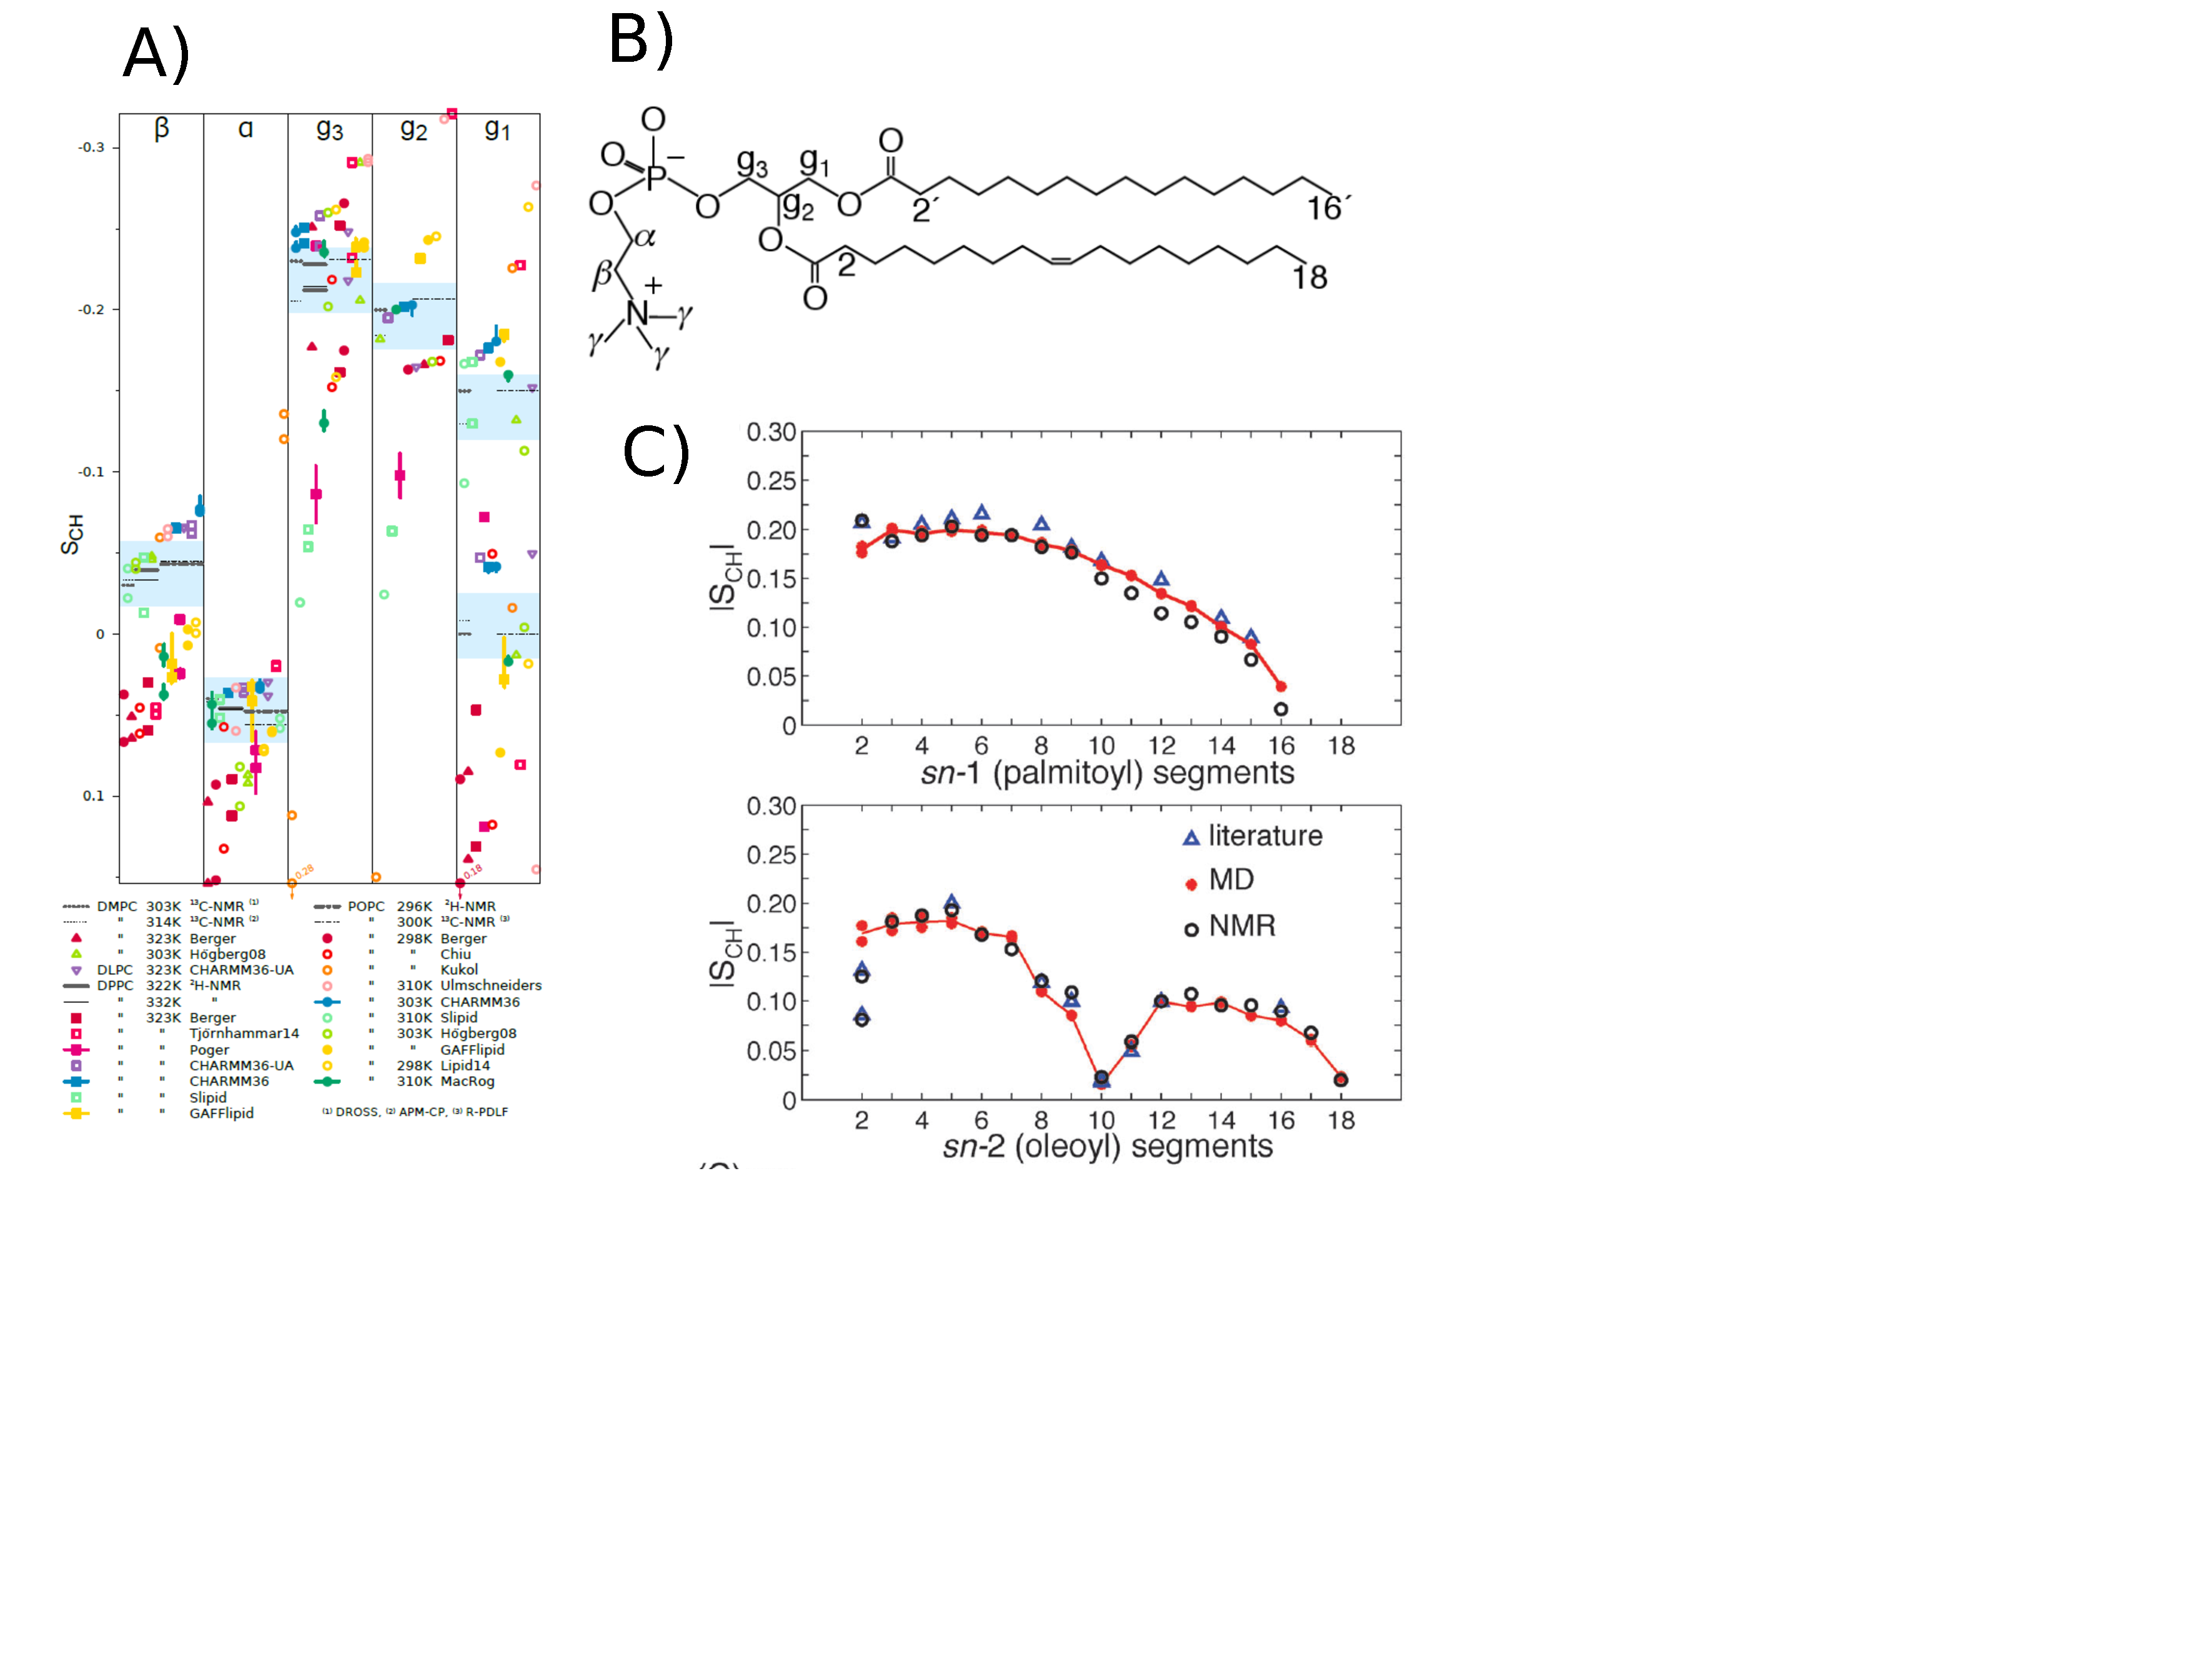
\includegraphics[width=12.2cm]{../Fig/allOPs.eps}
  \caption{\label{allOPs}
    A)  Order parameters from simulations and experimens for phosphatidylcholine headgroup and glycerol 
    backbone segments~\cite{botan15}. The blue shaded regions show the
    subjective sweetspots where the simulation data should fall to agree with experiments, 
    based on estimated quantitative accuracy of order parameter measurements by Botan et al.~\cite{botan15}.
    Adapted with permission from Botan et al. J. Phys. Chem. B. DOI:10.1021/acs.jpcb.5b04878 Copyright 2015 American Chemical Society.
    B) Chemical structure of 1-palmitoyl-2-oleoylphosphatidylcholine (POPC).
    C) Order parameters $|S_{{\rm CH}}|$ for POPC acyl chains 
    from $^1$H-$^{13}$C NMR at 300K (black dots)~\cite{ferreira13},
    from $^2$H NMR at 300K (blue triangles, literature)~\cite{seelig78,perly85} and 
    from MD simulations at 298K (red dots)~\cite{ferreira13}.
    Adapted from Ref.~\cite{ferreira13} with permission from the PCCP Owner Societies. 
    The experimental values shown in A):
    DMPC 303~K \cite{gross97},
    DMPC 314~K \cite{dvinskikh05a},
    DPPC 322~K \cite{gally75},
    DPPC 323~K \cite{akutsu81},
    POPC 296~K \cite{bechinger91}, and
    POPC 300~K \cite{ferreira13}.
    The force fields in A):
    Berger \cite{berger97},
    Hogberg08 \cite{hogberg08},
    Poger \cite{poger10},
    Ulmschneiders \cite{ulmschneider09},
    Kukol \cite{kukol09},
    Chiu \cite{chiu09},
    CHARMM36 \cite{klauda10},
    GAFFlipid \cite{dickson12},
    Slipid \cite{jambeck12},
    MacRog \cite{maciejewski14},
    Tj{\"o}rnhammar14 \cite{tjornhammar14},
    Lipid14 \cite{dickson14},
    CHARMM36-UA \cite{lee14}. 
    The interactive version of A) is available at  https://plot.ly/$\sim$HubertSantuz/72/lipid-force-field-comparison/.   
  }
\end{figure}


Experimental order parameter data for single component lipid bilayers are easily available in the literature~\cite{castro07,castro08,leftin11,marsh13,ferreira13,leftin13,leftin14,botan15}. 
The amount of data, especially from $^{13}$C NMR, has been also increasing of late~\cite{castro07,castro08,ferreira13,leftin13,leftin14}.
Further, changes of order parameters for all lipid segments have been measured various experimental
different conditions, like temperature \cite{seelig74,gally75,seelig77,douliez95}, 
hydration level \cite{bechinger91,ulrich94,mallikarjunaiah11,dvinskikh05a} and in the presense 
of charged objects~\cite{akutsu81,altenbach84,seelig87,scherer89}, 
cholesterol \cite{brown78,douliez95,ferreira13,leftin14} and proteins \cite{kuchinka89,roux90,leftin13}.
Since the comparison of order parameter responses between experiments and simulations
has not been much utilized, we will exemplify its potential by showing
the effect of Na$^+$ ions on choline order parameters and its relation to ion partition in 
simulations \cite{ionpaper} and experiments \cite{akutsu81,altenbach84,seelig87,scherer89}.

In this work we discuss only order parameters obtained from multilamellar samples, as they are  the closest experimental analogue to MD simulations with periodic boundary conditions. 
We do not discuss order parameters measured for other type of samples, such as 
bicelles~\cite{aussenac03,raffard00,sanders92}, or indirect measurements by using, e.g. relaxation
data~\cite{marbella15} since the comparison to the standard simulation setup is less straightforward.  



\subsection{Order parameters from $^2$H NMR experiments}\label{DopSECTION}

The absolute values of order parameters are connected to the quadrupolar splitting $\Delta \nu_Q$ 
in $^2$H NMR experiments through the equation 
\begin{equation}\label{HNMRop}
|S_{{\rm CD}}|=\frac{4}{3} \frac{h}{e^2qQ} \Delta \nu_{{\rm Q}}, 
\end{equation}
where $e$ is the elementary charge, $Q$ is the deuteron quadrupole moment and $h$ is the Planck's constant. 
The parameter $q$ is related to the largest electric field gradient and in practise its value is not known; 
therefore the static quadrupolar coupling constant $\frac{e^2qQ}{h}$ is defined, and its value is measured for 
different compounds in their solid state ($\Delta \nu_Q$ measurement from the system where order parameter is known to be 1). 
The value measured for different alkenes, $\frac{e^2qQ}{h}$=170 kHz is typically used in 
C-D order parameter measurements for lipids. The relation between order parameters 
and quadrupolar splittings then becomes $S_{{\rm CD}}=0.00784 \times \Delta \nu_{{\rm Q}}$.
With this relation the quadrupolar splittings reported in the literature can be translated to 
the order parameter values. For a review and more accurate description see, e.g. Ref.~\cite{seelig77c}.

For $^2H$ NMR measurements the CH$_2$ segments have to be labeled with deuterium.
This can be done specifically for a certain segment or for the several segments
simultaneously~\cite{davis83,bloom91,leftin11}. In the first case, it is known that the measured
order parameter (quadrupolar splitting) is related to the labeled segment.
In the latter case several order parameters (quadrupolar splittings) are simultaneously
measured which arise from all the labeled segments, however, it is not known 
which order parameter belongs to which CH$_2$ segment. Majority of the $^2H$ NMR data
in the literature are measured using samples with perdeuterated acyl chains \cite{leftin11,marsh13}
while also order parameter data from specifically deuterated lipids are available for 
several lipid types in various conditions~\cite{seelig74,seelig75,seelig77,seelig78,gally81,akutsu81,altenbach84,scherer89,kuchinka89,roux90,ulrich94,douliez95}.

\subsection{Order parameters from $^{13}$C NMR experiments}\label{CopSECTION}

The order parameter can be related to the dipolar splitting $\Delta \nu_\mathrm{CH}$ 
from $^{13}$C-$^1$H NMR experiment which is related to the effective dipolar 
coupling $d_\mathrm{CH}$ through a scaling factor depending on the used pulse 
sequence~\cite{hong95a,gross97,dvinskikh05a,ferreira13}. The effective dipolar 
coupling $d_{{\rm CH}}$ is then connected to the absolute value of order parameter through equation
\begin{equation}\label{CNMRop}
|S_{{\rm CH}}|=(\frac{D_{{\rm max}}}{2\pi})^{-1}d_\mathrm{CH},
\end{equation}
where $D_{{\rm max}} = \frac{\hbar \mu_0 \gamma_h \gamma_c}{4\pi\langle r_\mathrm{CH}^3 \rangle}$. 
$r_{{\rm CH}}$ is the C-H distance, $\mu_0$ is the vacuum permittivity, and $\gamma_h$ and $\gamma_c$ are 
the gyromagnetic constants for $^1$H and $^{13}$C nuclei. In contrast to Eq.~\ref{HNMRop}, all the parameters in 
Eq.~\ref{CNMRop} are in principle known. However, for the internuclear distance only the average $\langle r_{{\rm CH}} \rangle$ 
is known, but not the third moment $\langle r^3_{{\rm CH}} \rangle$. For this reason frequencies between 20.2-22.7 kHz have been used for
$\frac{D_{{\rm max}}}{2\pi}$~\cite{hong95a,gross97,dvinskikh05a,becker05,ferreira13,ferreira15}.

In contrast, specific labeling is not needed for $^{13}$C NMR experiments due the 
natural abundance of $^{13}$C.  Labeling can be, however, used to enhance the signal for a specific 
segment of interest~\cite{sivanandam09}. Order parameter measurements with $^{13}$C NMR are
2D experiments, the chemical shift being in the first dimension and dipolar coupling 
in the second~\cite{hong95a,gross97,dvinskikh05a,ferreira13}. The chemical shift depends on the local chemical environment and is different for each carbon segment. In the second dimension the dipolar coupling
(order parameter) corresponding to each chemical shift value is measured, and its value 
can be connected, in principle, to each carbon segment by using the chemical shift value.  
This is straighforward for hydrocarbon segments in choline, glycerol backbone, close to the 
double bonds, and in the beginning and the end of acyl chains due to their distinct chemical 
shift values~\cite{hong95a,gross97,dvinskikh05a,ferreira13,leftin14}.
Challenges occur in the acyl chain region, where chemical shift values 
of different segments are very close to each other~\cite{hong95a,gross97,dvinskikh05a,ferreira13,leftin14}. 
This issue has been solved by filtering the spectra by using partially deuterated lipids
and data from simulations to help the assigment~\cite{ferreira13,leftin14}. 


\subsection{Quantitative accuracy of experimental order parameter values}\label{QUANTaccuracySECTION}

It must be stressed that $^2$H NMR and $^{13}$C NMR are fully independent experiments since the deuterium quadrupolar splitting $\Delta \nu_Q$
and the dipolar splitting $d_{{\rm CH}}$ are different physical observables. In addition, the prefactors connecting the observables to the order 
parameter (Eqs.~\ref{HNMRop} and~\ref{CNMRop}) are independently measured. Further independent experiments are performed 
by measuring the $^1$H-$^{13}$C dipolar couplings using different pulse sequences~\cite{hong95a,gross97,dvinskikh05a,ferreira13} 
when the connection between dipolar splitting $\Delta \nu_{{\rm CH}}$ and effective dipolar coupling $d_\mathrm{CH}$ is different.

The quadrupole $\Delta \nu_Q$ and dipolar $d_{{\rm CH}}$ splittings can be measured with higher accuracy than
the prefactors connecting them to order parameters in Eqs.~\ref{HNMRop} and~\ref{CNMRop},
thus in practise the prefactors determine the quantitative accuracy of measured order parameters. 
Since the prefactors are determined independently in $^2$H and $^{13}$C NMR measurements,
the quantitative accuracy is best estimated by comparing the measured order parameter values
from different experiments.

These comparisons are done by several authors and generally show a very good 
agreement~\cite{gross97,dvinskikh05a,ferreira13,botan15,leftin14}.
Botan et al. collected literature values for PC lipid choline headgroup and glycerol backbone order parameters 
and suggested that order parameters are known with the accuracy of $\pm$0.02 for these segments in 
purified PC lipid bilayer samples~\cite{botan15} which agrees with the estimate of Gross et al~\cite{gross97}. 
Based on this estimation Botan et al. suggested sweet spots where choline and glycerol backbone order parameters from simulations should range, see Fig.~\ref{allOPs} A). Also acyl chain order parameters from different techniques 
are in good agreement when compared by several authors~\cite{gross97,dvinskikh05a,ferreira13,leftin14},
however the 0.02 accuracy might not be achieved for some segments.%\todo{Maybe specify to which ones?}.
The comparison by Ferreira et al.~\cite{ferreira13} for POPC acyl chains is also shown in Fig.~\ref{allOPs} C). 







\subsection{Qualitative accuracy of experimental order parameter values}

When order parameter changes are measured with varying conditions, like temperature \cite{seelig74,seelig77,douliez95}, 
hydration level~\cite{bechinger91,ulrich94,mallikarjunaiah11,dvinskikh05a}, presense of ions~\cite{akutsu81,altenbach84,seelig87,scherer89}, 
cholesterol~\cite{brown78,douliez95,ferreira13,leftin14} or proteins~\cite{kuchinka89,roux90,leftin13},
the prefactors connecting order parameters and measured couplings in Eqs.~\ref{HNMRop} and~\ref{CNMRop} can be considered 
to be unchanged. Therefore, accuracy of the measured change is determined by the accuracy of the splitting 
measurement, in contrast to the quantitative accuracy discussed in previous section. Here we refer to this 
as a qualitative accuracy. Due to the high resolution of splitting measurements, especially in $^2$H NMR, 
the qualitative accuracy is much higher than the quantitative accuracy.

The high qualitative accuracy of order parameter measurements is demonstrated in Figs.~\ref{opIONeffect} and~\ref{opDEHYDeffect}
showing the measured changes as a function of ion concetrations and hydration level, respectively.
Systematically observed order parameter decrease of choline $\alpha$ and $\beta$ segments due to penetrating 
positive charges~\cite{akutsu81,altenbach84,seelig87,scherer89} from $^2$H NMR are shown in Fig.~\ref{opIONeffect} A).
The quadrupole splittings reported in the original work~\cite{akutsu81} and corresponding order parameters 
are shown. The distinct quadrupolar splitting changes correspond to order parameter changes below 0.03 and 
0.05 units for $\beta$ and $\alpha$, respectively. Systematically observed increase for choline $\beta$ and $\alpha$
segments due to decreased hydration level are shown in Fig.~\ref{opDEHYDeffect}. 
A similar increase is observed for different phosphatidycholine lipids in slightly different temperatures by
different groups using both $^2$H NMR~\cite{bechinger91,ulrich94} and $^{13}$C NMR~\cite{dvinskikh05b}.
The results demonstrate the systematic changes only slightly above 0.01 units can be detected also with $^{13}$C NMR~\cite{dvinskikh05b}.

\begin{figure*}[]
%  \centering
  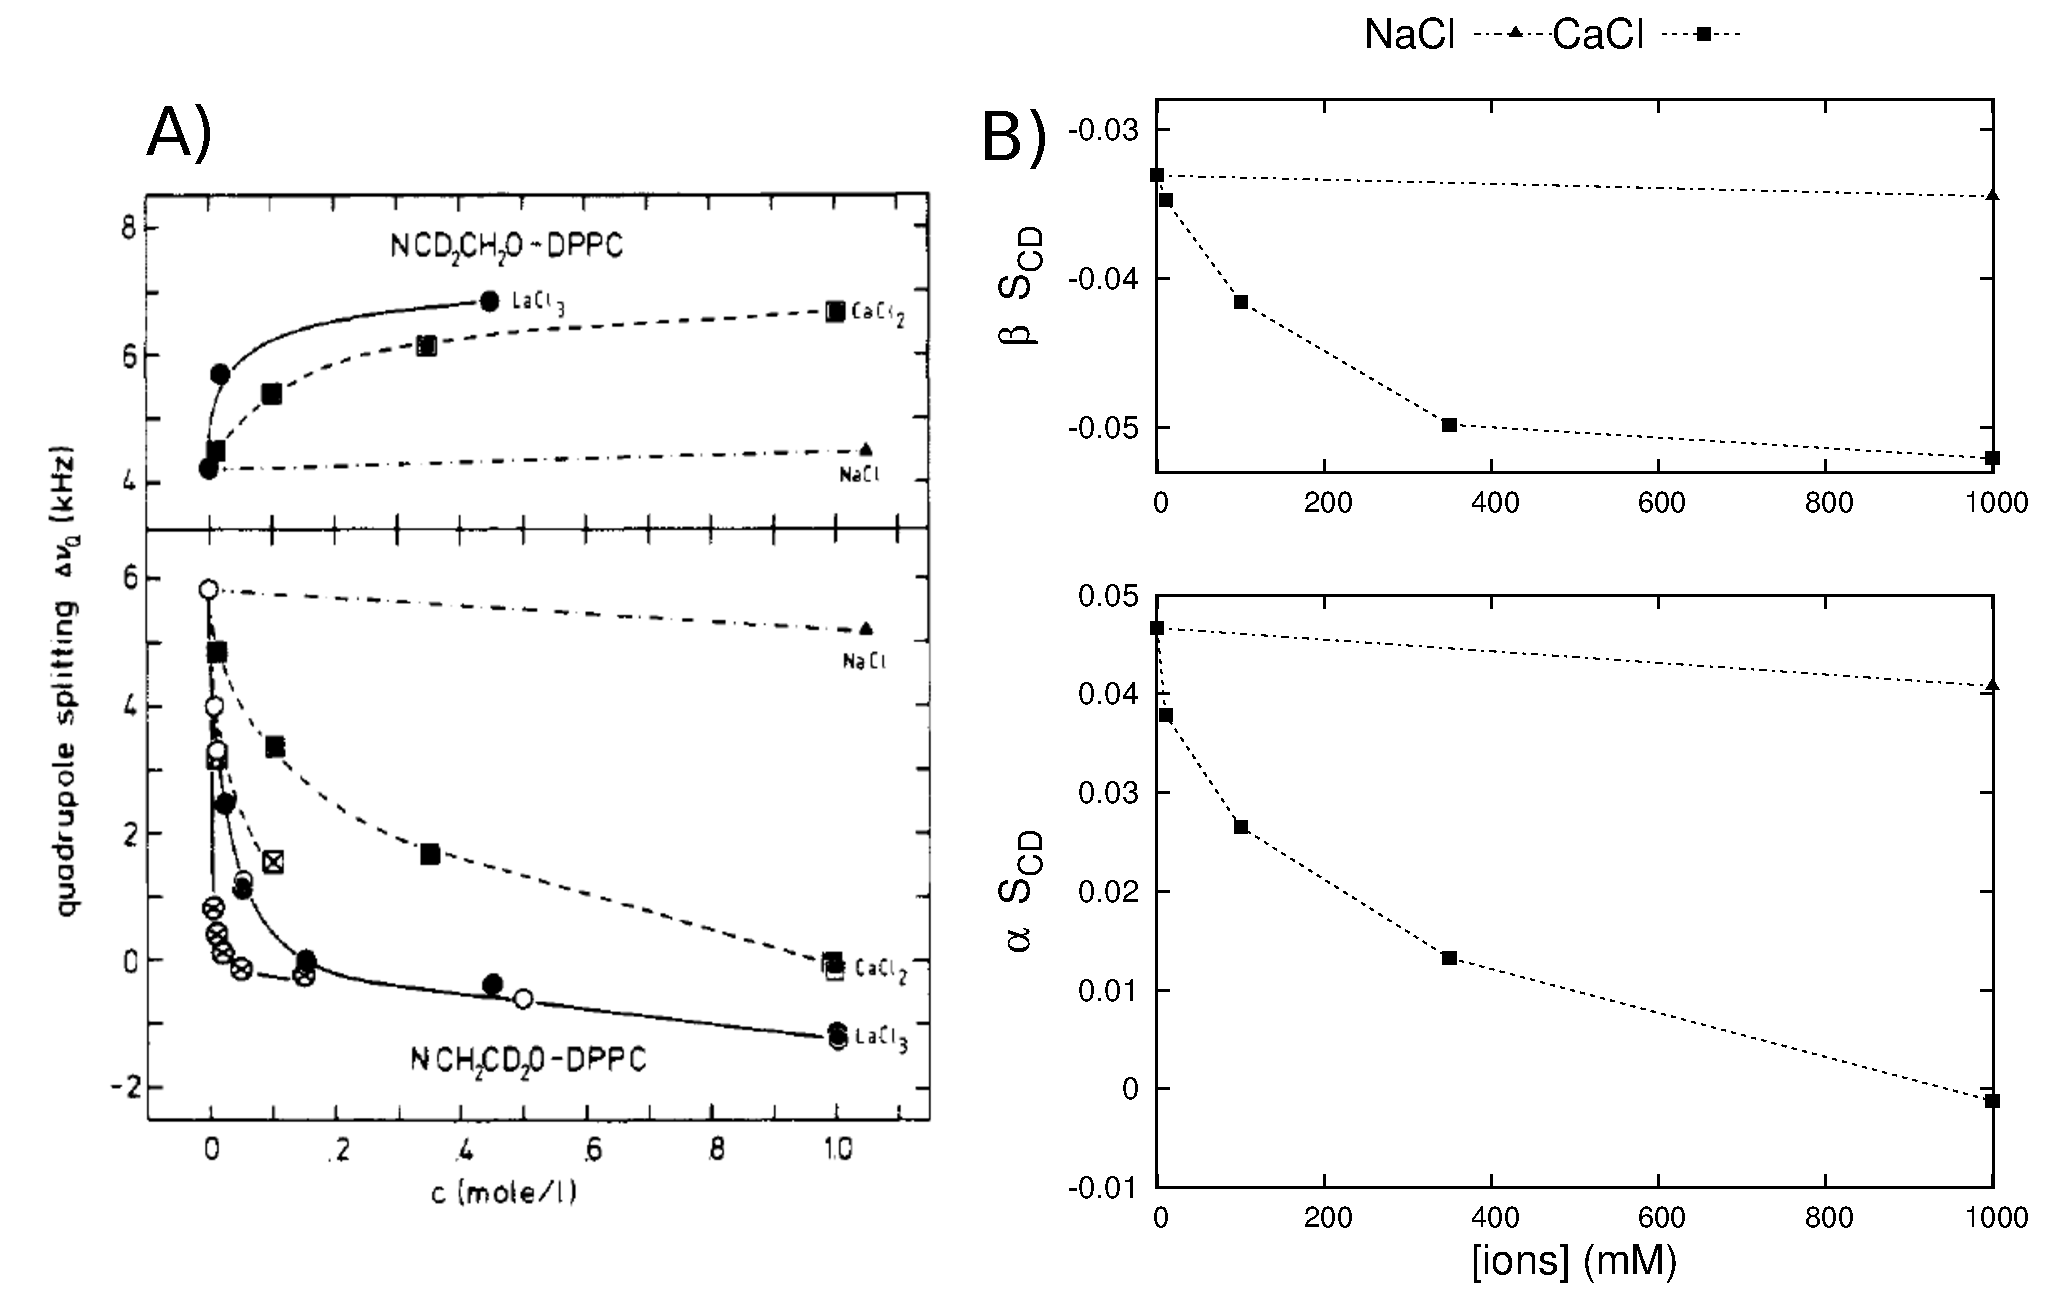
\includegraphics[width=12.2cm]{../Fig/QPandOPwithIONS.eps}
  \caption{\label{opIONeffect}
    A) Quadrupolar splittings of DPPC $\alpha$ and $\beta$ segments as a function of different 
    ion concetrations measured by Akutsu and Seelig with $^2$H NMR~\cite{akutsu81}. 
    Adapted with permission from Akutsu et al. Biochemistry {\bf 1981}, 20, 7366-7373. Copyright 1981 American Chemical Society.
    B) The measured quadrupolar splittings with NaCl and CaCl$_2$ translated to order parameters ($S_{{\rm CD}}=0.00784 \times \Delta \nu_{{\rm Q}}$). 
    The negative sign for $\beta$ order parameter is assigned according to more recent experiments~\cite{hong95a,hong95b,gross97} 
    (see also Ref.~\cite{botan15} and Section~\ref{signSECTION}). These changes were later shown to be consistent with the 
    addition of different charges into the bilayer, and the electrometer concept was introduced to measure the amount of charge 
    incorporated in the bilayer interface~\cite{akutsu81,altenbach84,seelig87,scherer89}.
  } 
\end{figure*}

\begin{figure}[]
%  \centering
  \includegraphics[width=8.6cm]{../Fig/OrderParameterDEHYDexp.eps}
\newline
  \caption{\label{opDEHYDeffect}
    Systematic increase of phosphatidylcholine $\alpha$ and $\beta$ order parameters with decreasing hydration level,
    observed with both $^2$H NMR~\cite{bechinger91,ulrich94} and $^{13}$C NMR~\cite{dvinskikh05b}.
    The negative sign for $\beta$ order parameter is assigned according to more recent experiments~\cite{hong95a,hong95b,gross97} 
    (see also Ref.~\cite{botan15} and Section~\ref{signSECTION}).
    The choline order parameter increase is related to the P-N vector tilting more parallel to the membrane plane~\cite{botan15}
    while relation between order parameter decrease and tilting more perpendicular has been suggested~\cite{scherer89}.
  } 
\end{figure}

In conclusion, the order parameter changes can be measured with very high accuracy,
thus even very small structural changes can be observed. Molecular models are necessary
to analyze the measured changes to avoid overinterpretation of minute changes observed in experiments.
For example, high concentration of cholesterol induces measurable changes (less than 2~kHz) to the DPPC $\alpha$ and $\beta$ 
quadrupolar splittings, however, the related structural changes are probably almost negligible~\cite{brown78,botan15}.


\subsection{Signs of order parameters}\label{signSECTION}

$^2$H NMR~\cite{seelig77c} and standard $^1$H-$^{13}$C NMR~\cite{hong95a,gross97,dvinskikh05a,ferreira13} measure 
only the absolute value of order parameter. However, two different $^1$H-$^{13}$C NMR techniques applied to eggPC~\cite{hong95a} 
and DMPC~\cite{hong95a,gross97} allow also the measurement of the sign.
The experiments report negative order parameters for almost all the segments, only $\alpha$ and $\gamma$ are positive.
Furthermore, the signs~\cite{hong95a,hong95b,gross97} and magnitudes~\cite{gally81,ferreira13,botan15} of choline headgroup 
and glycerol backbone order parameters are practically unaffected by the acyl chain contents of the bilayers. 
The results indicate that the order parameter signs for these segments can be assumed to be the same in all PC lipids in bilayer. 
On the other hand, positive signs for g$_1$, g$_3$ and C$_2$ have been reported by Aussenac et al.~\cite{aussenac03}, which has led to some confusion in the simulation community~\cite{hogberg06,hogberg08,signPOST}. 
However, these signs were not directly measured but extracted from the model used to interpret 
$^2$H NMR order parameters from DMPC bicelles~\cite{aussenac03}. Thus, it is reasonable to conclude that 
order parameters are negative for all segments except for $\alpha$ and $\gamma$, as 
directly measured with $^1$H-$^{13}$C NMR~\cite{hong95a,hong95b,gross97}.

%Even though the sign was not measurable with $^2$H NMR, the sign was believed to be negative for acyl chains because $\theta$ was expected to fluctuate 
%around 90$^o$ leading to negative order parameters~\cite{seelig77c}. This was later confirmed by using $^{13}$C NMR measurements~\cite{hong95a}. 
%Also MD simulations always produce negative order parameters for acyl chains.

In measurements of order parameter changes with respect to varying 
conditions~\cite{seelig74,seelig77,bechinger91,ulrich94,mallikarjunaiah11,dvinskikh05a,akutsu81,altenbach84,seelig87,scherer89,brown78,douliez95,ferreira13,leftin14,kuchinka89,roux90,leftin13} 
only the absolute values are measured. However, the experiments are usually done by gradually changing the conditions and systematic 
order parameter responses are observed~\cite{akutsu81,altenbach84,bechinger91,ulrich94,dvinskikh05b,mallikarjunaiah11,ferreira13} 
(see also Figs.~\ref{opIONeffect} and~\ref{opDEHYDeffect}), indicating that sudden changes of sign do not occur. 
On the other hand, the large amount of bound positive charge may decrease the $\alpha$ carbon order parameter below zero as demonstrated by the spectra measured by Altenbach and Seelig~\cite{altenbach84} for POPC with high concetrations of CaCl$_2$,
shown in Fig.~\ref{qsCACLeffect}.
\begin{figure}[]
%  \centering
  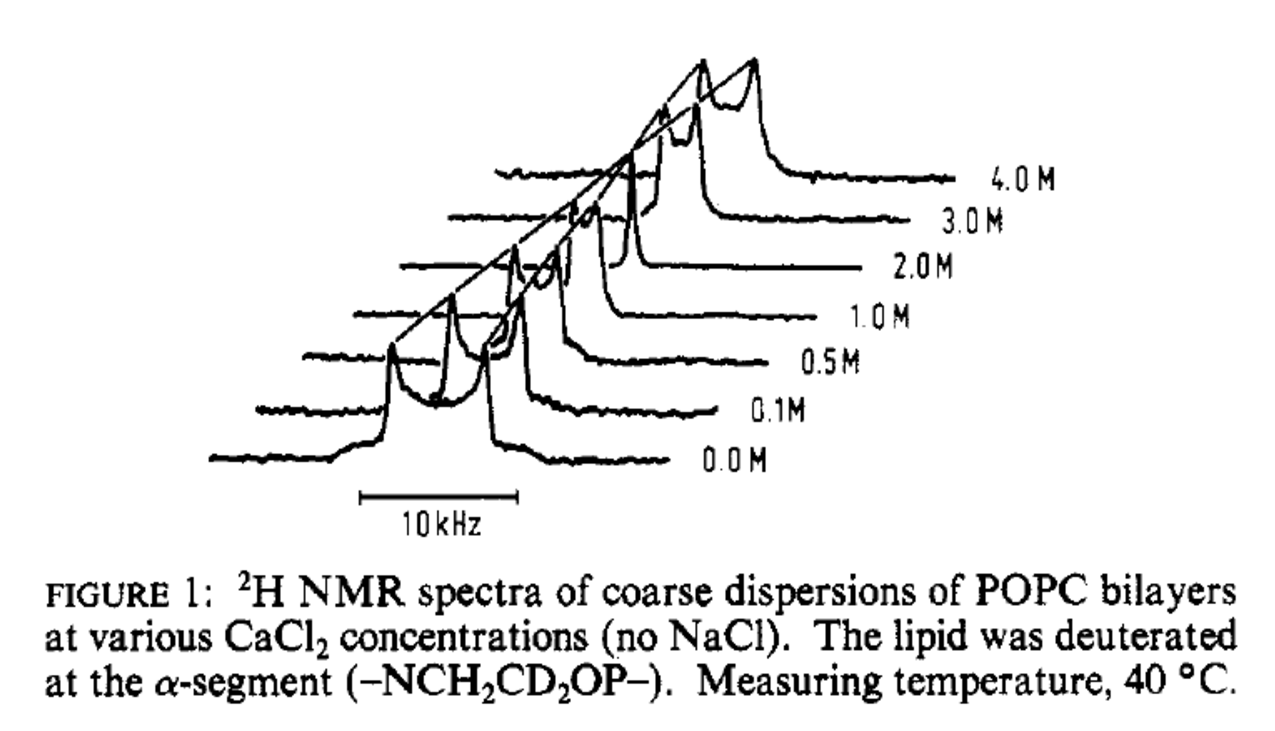
\includegraphics[width=8.6cm]{../Fig/QUADsplitCACLeffect.eps}
\newline
  \caption{\label{qsCACLeffect}
    Quadrupolar splitting $\Delta \nu_Q$ for $\alpha$ segment in POPC as a function of CaCl$_2$ concentration measured by Altenbach and Seelig~\cite{altenbach84} at 313~K.
    The splitting is related to the order parameter as $S_{{\rm CD}}=0.00784 \times \Delta \nu_Q$. 
    More recent studies show that the $\alpha$ order parameter is positive in the absense of CaCl$_2$~\cite{hong95a,hong95b,gross97}.
    Thus, the most obvious interpertation is that the $\alpha$ order parameter decreases to zero when CaCl$_2$ concentration reaches 2.0M, and 
    becomes increasingly negative with further addition of CaCl$_2$. Reprinted with permission from Altenbach and Seelig, Biochemistry, 23, 3913 (1984). Copyright 1984 American Chemical Society.    
  } 
\end{figure}



\subsection{Forking of order parameters}

The order parameters for two C--H bonds in the same CH$_2$ segment are equal for the most lipid 
segments~\cite{seelig74,seelig77,seelig78,gally81,gross97,dvinskikh05a,ferreira13}.
Exceptions in a fluid PC lipid bilayer are g$_1$, g$_3$, and  the C$_2$ carbon in the \textit{sn}-2 chain 
segments as observed with both $^2$H NMR~\cite{seelig75,seelig78,engel81,gally81} and 
$^1$H-$^{13}$C NMR techniques~\cite{gross97,dvinskikh05a,ferreira13}, see also Fig.~\ref{allOPs}.
We call this phenomena {\it forking}, as done also previously to avoid confusion with splittings measured with NMR~\cite{botan15}.

The forking has been studied in detail with $^2$H NMR techniques by separately deuterating the 
R or S positions in CH$_2$ segments in order to assign order parameters to correct hydrogens \cite{gally81,engel81}.
These studies also show that the forking arises from differently sampled orientations 
of the two C--H bonds, not from two separate populations of lipid conformations~\cite{engel81,gally81}.
This means that realistic atomistic resolution molecular model has to reproduce the forking 
correctly and that the isomeric positions of hydrogens must be taken into account when calculating
order parameters from simulations~\cite{botan15}.



\subsection{Order parameters from simulations}

Since all the atom coordinates are available from a molecular dynamics simulation trajectory,
the order parameters can be calculated directly from the definition in Eq.~\ref{orderP}.
The ensemble average is taken over the simulation time and all the molecules in simulation.
The hydrogen positions can be generated post-simulationally based on heavy atoms positions and the 
known hydrocarbon geometries for united atom simulations without explicit hydrogens 
by creating a trajectory with added hydrogens~\cite{ollila07a,botan15} or by using equations to directly calculate 
order parameters~\cite{tieleman97,vermeer07}. The first approach is appropriate for accurate 
structural studies since it allows to analyse forking in contrast to the latter technique.

The difference in the analysis methods for the forked segments is most likely the reason for 
diverging choline and glycerol backbone order parameters reported for the same models by different 
authors~\cite{poger12,botan15}. Also different order parameters for C--H segments attached to double 
bond are reported for the same model~\cite{bachar04,ollila07a} due to a bug in a widely-used version of 
the {\it g\_order} program in the Gromacs package. The {\it g\_order} program also prints -S$_{{\rm CH}}$, 
which is the most likely reason for the reported positive order parameters for acyl chains in some studies~\cite{ekkabut07}.
When these technical issues are taken into account, the different order parameters calculations from simulations are 
in good agreement.

The statistical error for order parameters is estimated by using the error of the mean for time blocks~\cite{ollila07a},  
independent simulations~\cite{poger12} and different lipids~\cite{botan15}. All these approaches yield a maximum error of $\sim \pm$0.01.

It was recently pointed out that the sampling of individual dihedral angles might be very
slow compared to the typical (100~ns) simulation timescales~\cite{vogel12}.
This result raises a question if the molecules sample the full phase phase
during typical simulation time scales. On the other hand, another recent study showed
that the slowest rotational auto-correlation function observed (for g$_1$ segment) 
in the Berger model reached a plateau ($S_\mathrm{CH}^2$) after $\sim$200~ns
and its relaxation was significantly too slow compared to NMR relaxation experiments~\cite{ferreira15},
see Fig \ref{correlationF}. 
This indicates that the typical simulation times are long enough for full conformational 
phase space sampling for the models with realistic dynamics~\cite{ferreira15}.



\subsection{Comparison between order parameters from simulations and experiments}\label{OPcompSECTION}

The acyl chain order parameters are compared between simulations and experiments since the early days of lipid bilayer simulations~\cite{ploeg82,egberts88,stouch93,egberts94,essex94,robinson94,hyvonen95,kothekar96,tieleman96,shinoda97,berger97,tieleman97,klauda08b}. 
Good agreement has been generally found~\cite{berger97,hogberg08,poger10,ulmschneider09,kukol09,chiu09,klauda10,dickson12,jambeck12,chowdhary13,maciejewski14,tjornhammar14,dickson14,lee14}.
except for the C$_2$ segment of the {\it sn-2} chain having low magnitude and significant forking in all PC lipids, in constrast to C$_2$ of the chain linked to
{\it sn}-1~\cite{seelig74,seelig75,gross97,dvinskikh05a,ferreira13}, for example see Fig.~\ref{allOPs} C). 
This feature is, however, not analyzed or not reproduced for several lipid models~\cite{hogberg08,siu08,chiu09,kukol09,ulmschneider09,jambeck12,dickson12,chowdhary13,tjornhammar14,maciejewski14}.
Some models report the small order parameter for C$_2$,  but the forking is not correctly reproduced 
or analyzed~\cite{siu08,klauda10,chowdhary13,dickson14}.
Among all studied force fields, the united atom CHARMM36 is closest to the experimental results~\cite{lee14}.

Also acyl chain order parameter changes with varying conditions are compared between simulations and experiments
by several authors. Experimentally observed order parameter increase with cholesterol 
concentration~\cite{dufourc84,lafleur90,douliez95,urbina95,vermeer07,ferreira13} and dehydration~\cite{mallikarjunaiah11,dvinskikh05b} 
is observed also in simulations~\cite{mashl01,hogberg06,vermeer07,zhu07,lim12,ferreira13,jambeck13,madej15},
as well as the temperature induced order parameter decrease~\cite{douliez95,zhuang14}.
A more careful comparison reveals, however, that the temperature and dehydration effects are slightly underestimated in simulations 
compared to experiments~\cite{hogberg06,zhuang14}. Also cholesterol effects to DMPC bilayer are underestimated in the CHARMM36 model~\cite{lim12},
while Slipids~\cite{jambeck13} and Amber Lipid14~\cite{madej15} models show satisfactory agreement.
The comparison of a Berger/H{\"o}ltje~\cite{berger97,holtje01} based model to the extensive data set with 
various POPC/cholesterol mixtures shows good agreement with experiments for low cholesterol concetrations, 
however, the agreement gets worse for cholesterol concentration $\ge$ 34\%~\cite{ferreira13}. 
A recent comparison of the Amber Lipid14 model to the same experimental data shows significantly better 
agreement, althought slight overestimation of the ordering effect is observed with cholesterol concentration $\ge$ 34\%~\cite{madej15}, 
as shown in Fig.~\ref{cholTAILmadej}. The orientation of cholesterol ring structure in saturated or monounsaturated bilayers
is reasonable in all models \cite{vermeer07,lim12,ferreira13,madej15}, 
however, the cholesterol acyl chain exhibits too low order parameters in the Berger/H{\"o}ltje~\cite{berger97,holtje01} 
based model \cite{ferreira13} and too much forking in Amber Lipid14~\cite{madej15}, while CHARMM36 reproduces experiments well~\cite{lim12}. 
\begin{figure*}[]
%  \centering
  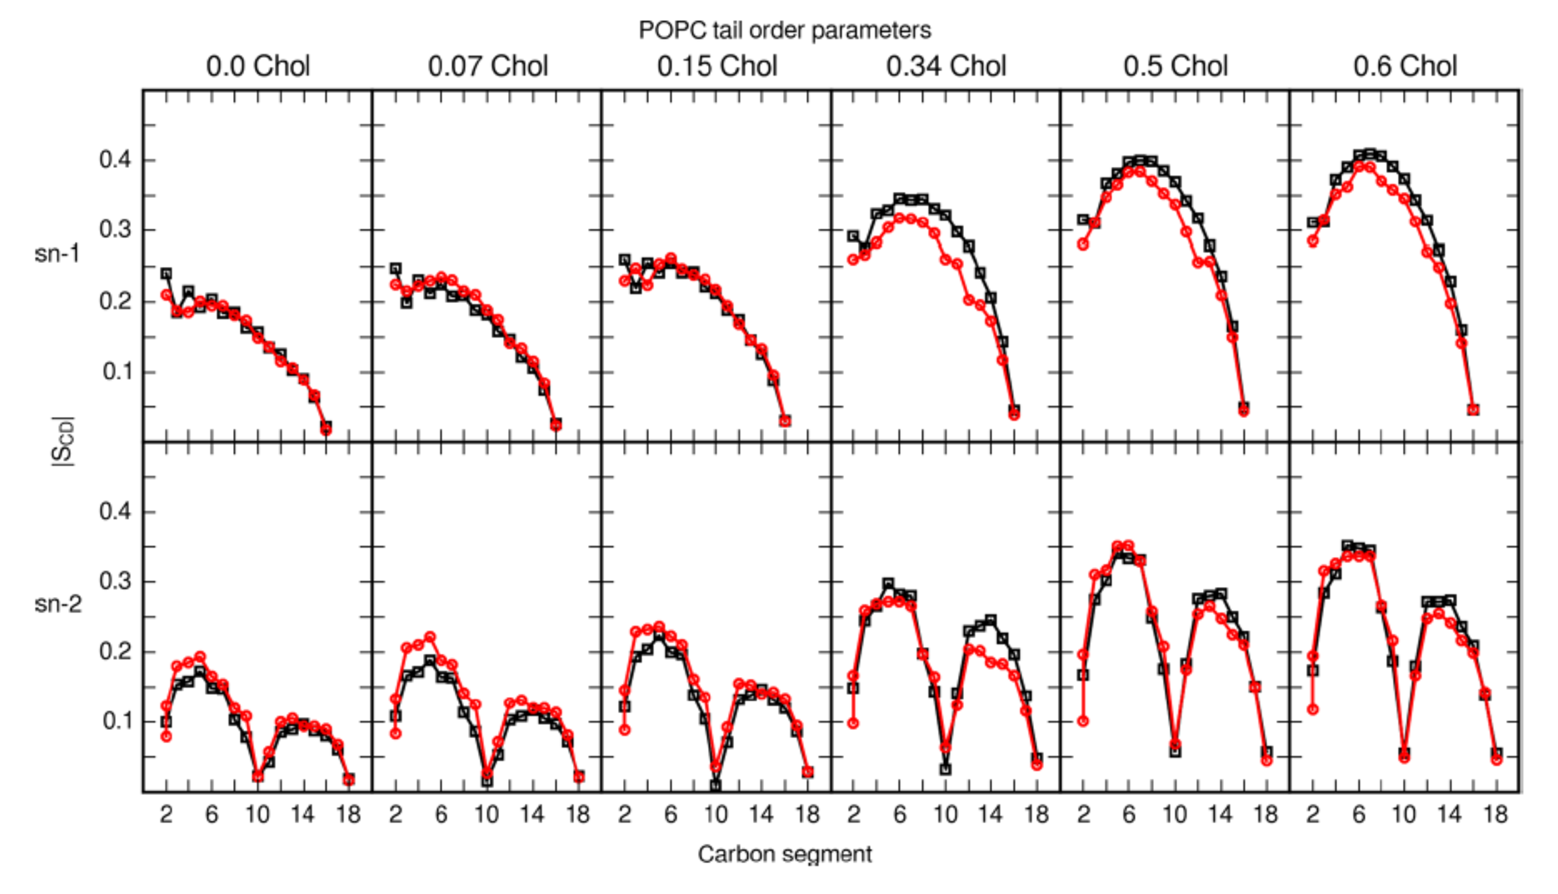
\includegraphics[width=12.2cm]{../Fig/cholTAILmadej.eps}
\newline
  \caption{\label{cholTAILmadej}
    Cholesterol effect on acyl chain order parameters compared between the Amber Lipid14 model (black squares)~\cite{madej15} and experiments (red circles)~\cite{ferreira13}
    showing significantly better agreement than Berger/H{\"o}ltje based model compared by Ferreira et al. \cite{ferreira13} to the same experimental data.
    Reprinted with permission from Madej et al. {\bf 2015}, 119, 12424-12435. Copyright 2015 American Chemical Society.
  } 
\end{figure*}


The dip of the acyl chain order parameter profile due to double bonds is generally reproduced by different simulation  models~\cite{hyvonen97,hyvonen97b,feller97,saiz01,huber02,feller02,bachar04,rog04,hyvonen05,ollila07a,dickson12,klauda10,klauda12,ferreira13,jambeck13,lee14,dickson14}. 
The particularly good agreement, often achieved for the oleyl chain in POPC bilayer with one {\it cis} double bond, is demonstrated in Fig.~\ref{allOPs} C).
Also the further order parameter decrease due to multiple double bonds (polyunsaturation)~\cite{hyvonen97,hyvonen97b,saiz01,huber02,feller02,bachar04,hyvonen05,ollila07a,klauda12} 
is usually well reproduced, as demonstrated in Fig. \ref{polyunsat} for Berger~\cite{berger97} based model with double bond description by Bachar et al.~\cite{bachar04}.
Also difference between {\it cis} and {\it trans} double bonds can be reproduced in MD simulations \cite{kulig15b}.
\begin{figure}[]
%  \centering
  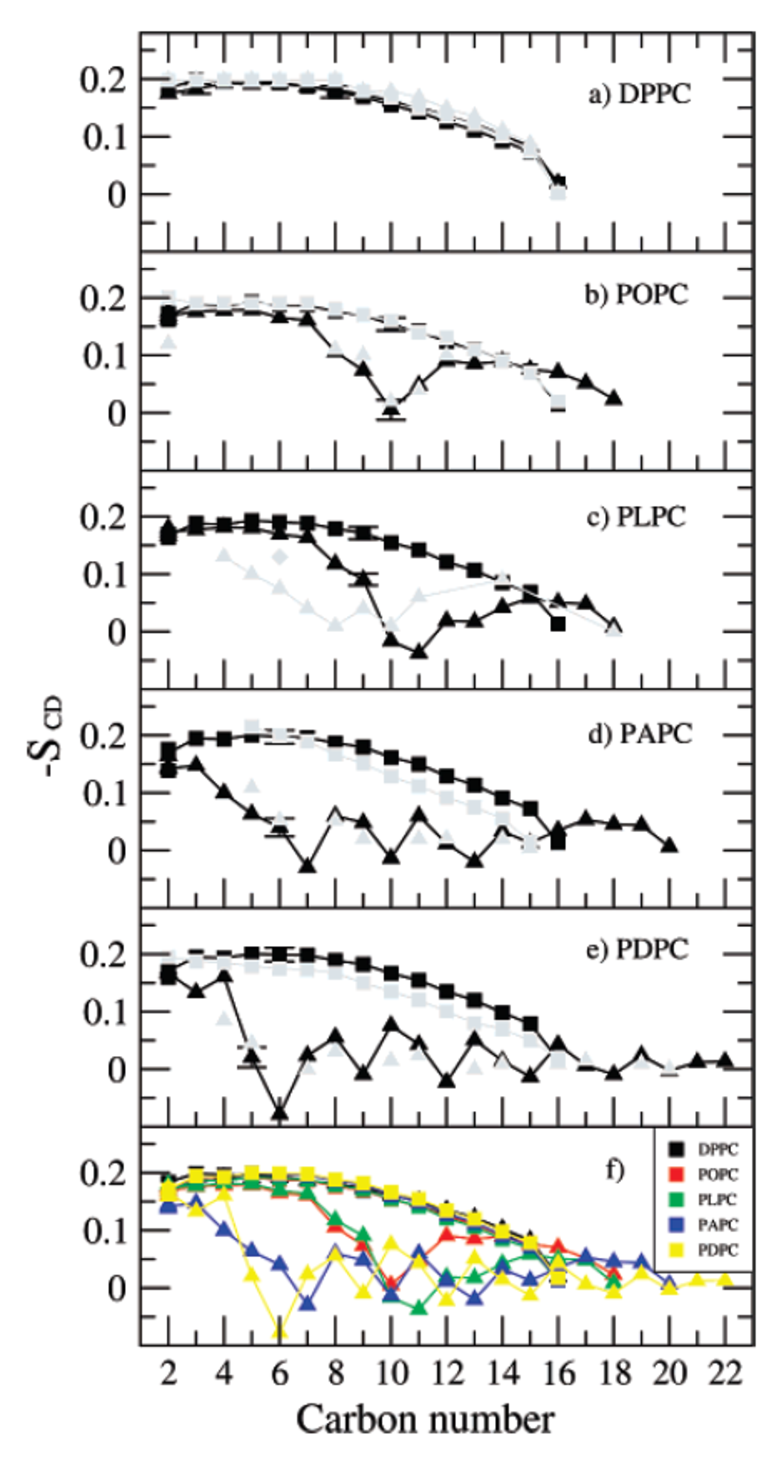
\includegraphics[width=7.5cm]{../Fig/polyunsat.eps}
\newline
  \caption{\label{polyunsat}
   Figure comparing order parameters in polyunsaturated acyl chains between simulations and experiments~\cite{ollila07a}.
   Order parameters for the sn-1 (squares) and sn-2 (triangles)
   chains of (A) DPPC, (B) POPC, (C) PLPC, (D) PAPC, and (E) PDPC.
   Simulation results are shown in full black, and experimental results
   for comparison in gray. Additionally, part F summarizes the data for
   all bilayers from the simulations. Experimental order parameters were
   chosen for comparison as follows. The order parameters for DPPC (T=323K) 
   are based on studies by Petrache et al. \cite{petrache00} whereas the
   experimental S$_{{\rm CD}}$ values for PDPC and for the sn-1 chain of POPC (T=310 K) 
   are based on studies by Huber et al. \cite{huber02} For the sn-1 chain of
   PDPC, the data set at 310 K is obtained by linearly interpolating
   between data at 303 and 323 K, whereas for the sn-2 chain the data at
   303 K are presented \cite{huber02}. Experimental values for the sn-2 chain of POPC
   are based on studies by Seelig et al. \cite{seelig78} A single experimental value is
   available also for the sn-2 chain of the PLPC bilayer at 313 K
   (diamond) \cite{baenziger91} to compare with our simulated order parameters for PLPC.
   Together with PLPC, there are also experimental results for PiLPC (T=313K) \cite{baenziger91}. 
   Experimental order parameters for the sn-1 and sn-2 chains
   of PAPC (T=303 K) are based on quadrupole splittings measured by
   Rajamoorthi et al. \cite{rajamoorthi91}. For the sn-1 chain the monotonic decrease through
   the acyl chain is expected. For the sn-2 chain, values are fitted such
   that the agreement is as good as possible.
   Reprinted with permission from Ollila et al. J. Phys. Chem. B, {\bf 2007}, 111, 3139-3150. Copyright 2007 American Chemical Society.
  } 
\end{figure}


In contrast to acyl chains, the glycerol backbone and choline order parameters are not routinely
compared between simulations and experiments. In most comparisons the experimentally available signs,
stereospecific labeling and high accuracy are not fully exploited~\cite{shinoda97,hogberg06,klauda10,poger12,dickson12,botan15,hogberg08,kapla12}.
These issues were recently dicussed by Botan et al. who also compared order parameters 
between 13 different simulation models and experiments~\cite{botan15}. The results, shown also in Fig.~\ref{allOPs} A),
reveal significant differences between models and experiments, and none of the available models
reproduces all order parameters within experimental error.
On the other hand, experimentally observed choline order parameter increase with 
dehydration~\cite{bechinger91,ulrich94,dvinskikh05b} and decrease due to cation 
penetration~\cite{akutsu81,altenbach84} were reproduced in simulations~\cite{botan15,ionpaper}.
However, especially the effect induced by Na$^+$ ion penetration is strongly overestimated
in several models which arises most likely from an artificially high partition coefficient~\cite{ionpaper},
as also demonstrated in Fig.~\ref{changesDUEna}.
The effect of cholesterol on glycerol backbone and choline is overestimated
by the Berger/H{\"o}ltje based \cite{ferreira13} and Amber Lipid14 \cite{madej15} models 
while CHARMM36 and MacRog performed better~\cite{botan15}. 
\begin{figure*}[]
%  \centering
  \includegraphics[width=12.2cm]{../Fig/changesDUEna.eps}
\newline
  \caption{\label{changesDUEna}
    Changes in choline order parameters (left column) and ion density distributions (right column)
    as a function of NaCl concentration. Significant order parameter
    reduction and Na$^+$ partition is observed with Berger model while only modest order parameter change
    and ion parition observed with CHARMM36. The results are in line with the electrometer concept
    connecting the ion partition and choline order parameters changes~\cite{akutsu81,altenbach84,seelig87,scherer89}.
    Consequently, the results show that Na$^+$ partition is significantly overestimated in the Berger model. 
    For more discussion see \cite{ionpaper}.
  } 
\end{figure*}

In conclusion, the acyl chain order parameters and their qualitative changes are 
generally well described in atomistic MD models, except for C$_2$ segment in {\it sn}-2.
However, all models have difficulties with varying severity to correctly describe 
the glycerol backbone and choline order parameters.



\subsection{Interplay between simulations and NMR order parameters: Validation and interpretation}\label{OPinterplay}

Since the acyl chain order parameters from MD models generally 
agree with experiments for single component lipid bilayers in full hydration, 
the conformations sampled in simulations
can be considered as realistic atomistic resolution structures for 
the acyl chains (except for the C$_2$ segment in the {\it sn}-2 chain).
As also the acyl chain rotational dynamics has the correct order of magnitude 
(see Section~\ref{dynamicsSECTION}), the dynamical nature of 
hydrophopic region of lipid bilayers seen in simulation videos
can be considered as a realistic representation of the system. 
This is significant advancement to the traditional static structural 
models~\cite{seelig74,schindler75,seelig78,baenziger91}.
Since lipid bilayers are considered as a simple models for cell- and other 
biological membranes, the intuitive understanding of their dynamical nature 
has a significant impact on biomembrane physics and chemistry. 

Also more detailed structural interpretation has been succesfull for
acyl chain region, especially for order parameter decrease due to {\it cis} double
bonds~\cite{feller02,huber02,eldho03,stillwell03,gawrisch03,bachar04,ollila07a}.
From NMR experiments alone it was not possible to judge if 
the order parameter decrease arises from the reduced chain order or the changes in 
average $\theta$ angle in Eq.~\ref{orderP}~\cite{stillwell03,gawrisch03}.
The interpretation of NMR experiments with the help of MD simulations revealed that
double bonds, indeed, decrease the chain order due to the flexible dihedral
potentials next to the rigid double bonds~\cite{feller02,huber02,eldho03,stillwell03,gawrisch03,bachar04,ollila07a}.

The acyl chain order parameter increase and related bilayer thickening with cholesterol 
concentration~\cite{vermeer07,zhu07,lim12,ferreira13,jambeck13,madej15},
dehydration~\cite{hogberg06,mashl01} and reduced temperature~\cite{zhuang14} are qualitatively reproduced 
by simulations giving intuitive visualizations for these effects. However, the order parameter
changes are often under- or overestimated \cite{hogberg06,lim12,zhuang14,ferreira13}, thus
it is not clear how well the models can be used for atomistic resolution intepretation of these changes.
For example, delicate lipid-cholesterol interactions are known to induce liquid-ordereded and liquid-disordered
phase coexistence \cite{ipsen87}. To give atomistic resolution interpretation for this phenomena \cite{rog09,somerharju09,rog14,sodt14}, 
the atomistic resolution structures and interactions should be correct, which does not seem to the case for 
several models~\cite{lim12,ferreira13,madej15}.

Simulation studies have also predicted changes in the acyl chain region which are yet to be experimentally 
confirmed, e.g. order parameter decrease due to lipid oxidation and changes in order parameter sign in oxidized 
acyl chain~\cite{ekkabut07}. %These are actually confirmed but not published yet. 

The usability of MD models for structural interpretation decrease closer to the interfacial region since the
experimental glycerol backbone, choline headgroup and {\it sn}-2 C$_2$ segment order parameters are 
not usually reproduced within experimental error, as discussed in the previous section. 
The forking and low order parameter values for C$_2$ in the {\it sn}-2 are related
to the parallel orientation of the chain respect to membrane normal~\cite{schindler75,seelig75}
which is suggested to have significant contribution e.g. to membrane electrostatic potential~\cite{gawrisch92}
and acyl chain extended conformations~\cite{kinnunen12}.
Also the atomistic resolution structures sampled by glycerol backbone and choline headgroup are not yet fully 
resolved~\cite{gally75,seelig77,strenk85,akutsu91,bruzik97,Semchyschyn04}.
Unfortunately the accuracy of atomistic resolution models is not yet sufficient to solve these issues.
However, the modeling of interfacial region structure has been getting more attention lately~\cite{klauda10,prakash10,dickson12,chowdhary13,botan15}, 
thus higher quality models may be expected.  

On the other hand, the increase of choline $\alpha$ and $\beta$ order parameters with dehydration 
and decrease with cation penetration were correctly reproduced by several models, 
despite of inaccurate choline structures~\cite{botan15,ionpaper}. The order parameter increase
was related to the choline P--N vector tilting more parallel to the membrane normal~\cite{botan15}
and order parameter decrease to the cation binding affinity~\cite{ionpaper}. 
The observations are in line with previous studies on charge penetration~\cite{akutsu81,altenbach84,seelig87,scherer89}.
However, choline structural changes due to cholesterol or ion concentration are significantly overestimated
in several models~\cite{ferreira13,botan15,ionpaper,madej15}, especially Na$^{+}$ binding affinity~\cite{ionpaper} (see also Fig.~\ref{changesDUEna}). 
The artificial specific Na$^{+}$  binding induces effectively postively charged membrane which may easily
lead to errorneous conclusion due to dominant contribution of electrostatics for various phenomena.

In conclusion, the atomistic resolution MD simulations are invaluable in understanding the 
structural details and their changes in acyl chain region. However, in applications where 
lipid interfacial region structure, energetics, electrostatics or ion distributions have significant role,
the potential artefacts arising from simulation models must be cafefully taken into account.
A typical example of such application would be a study of interactions between charge containing protein in solution
and lipid bilayer, simulated in physiological salt concentration~\cite{arkhipov13,kaszuba15}.


\section{C-H bond rotational dynamics from spin relaxation rates and simulations}\label{dynamicsSECTION}

\subsection{Definition and properties of rotational auto--correlation function}
The second order auto-correlation function for the reorientation of the C--H chemical bond axis is defined as
\begin{equation}\label{gt}
g(\tau) = \langle P_2[\vec{\mu}(t)\cdot\vec{\mu}(t+\tau)]\rangle,
\end{equation} 
where $P_2$ denotes the second Legendre polynomial, $P_2(\xi) = 1/2 (3\xi^2 - 1)$, $\vec{\mu}(t)$ is the unitary vector having the 
direction of the C--H bond at time $t$, and the angular brackets denote a time-average. 
For randomly oriented lamellar structures this auto--correlation is connected to the experimentally 
measurable spin relaxation rates through its Fourier transformation called spectral density~\cite{harris86}.
\begin{equation}\label{FT}
j(\omega) =  2\int_0^{\infty} \cos(\omega \tau) g(\tau) d\tau.
\end{equation}

The auto--correlation function for bond orientations always decays to zero
with long enough time scales in randomly oriented multilamellar samples due to the
diffusion between differently oriented bilayer regions. 
However, the relaxation processes occur in two distinct timescales and the auto--correlation function
can be written as a product of two independent functions~\cite{halle81,ferreira15}
\begin{equation}\label{corrF}
g(\tau)=g_{\rm{f}}(\tau) g_{\rm{s}}(\tau),
\end{equation}
where $g_{\rm{f}}(\tau)$ describes the fast decay (faster than $\sim \mu$s) due  
to the lipid rotation within bilayer plane and $g_{\rm{s}}(\tau)$ describes the slow motions (slower than $\sim \mu$s)
from the diffusion between differently oriented bilayer regions.
The correlation time of 4.2~ms for the slow decay was estimated from the spin-lattice relaxation rates in 
rotating frame $R_{1\rho}$, measured with different nutation frequencies for multilamellar POPC sample at 300K~\cite{ferreira15}.
The full auto--correlation decaying to zero, including the contribution from the magic angle spinning (MAS) in kHz region~\cite{nowacka10},
is illustrated in Fig.~\ref{correlationF}. 

\begin{figure}[]
%  \centering
  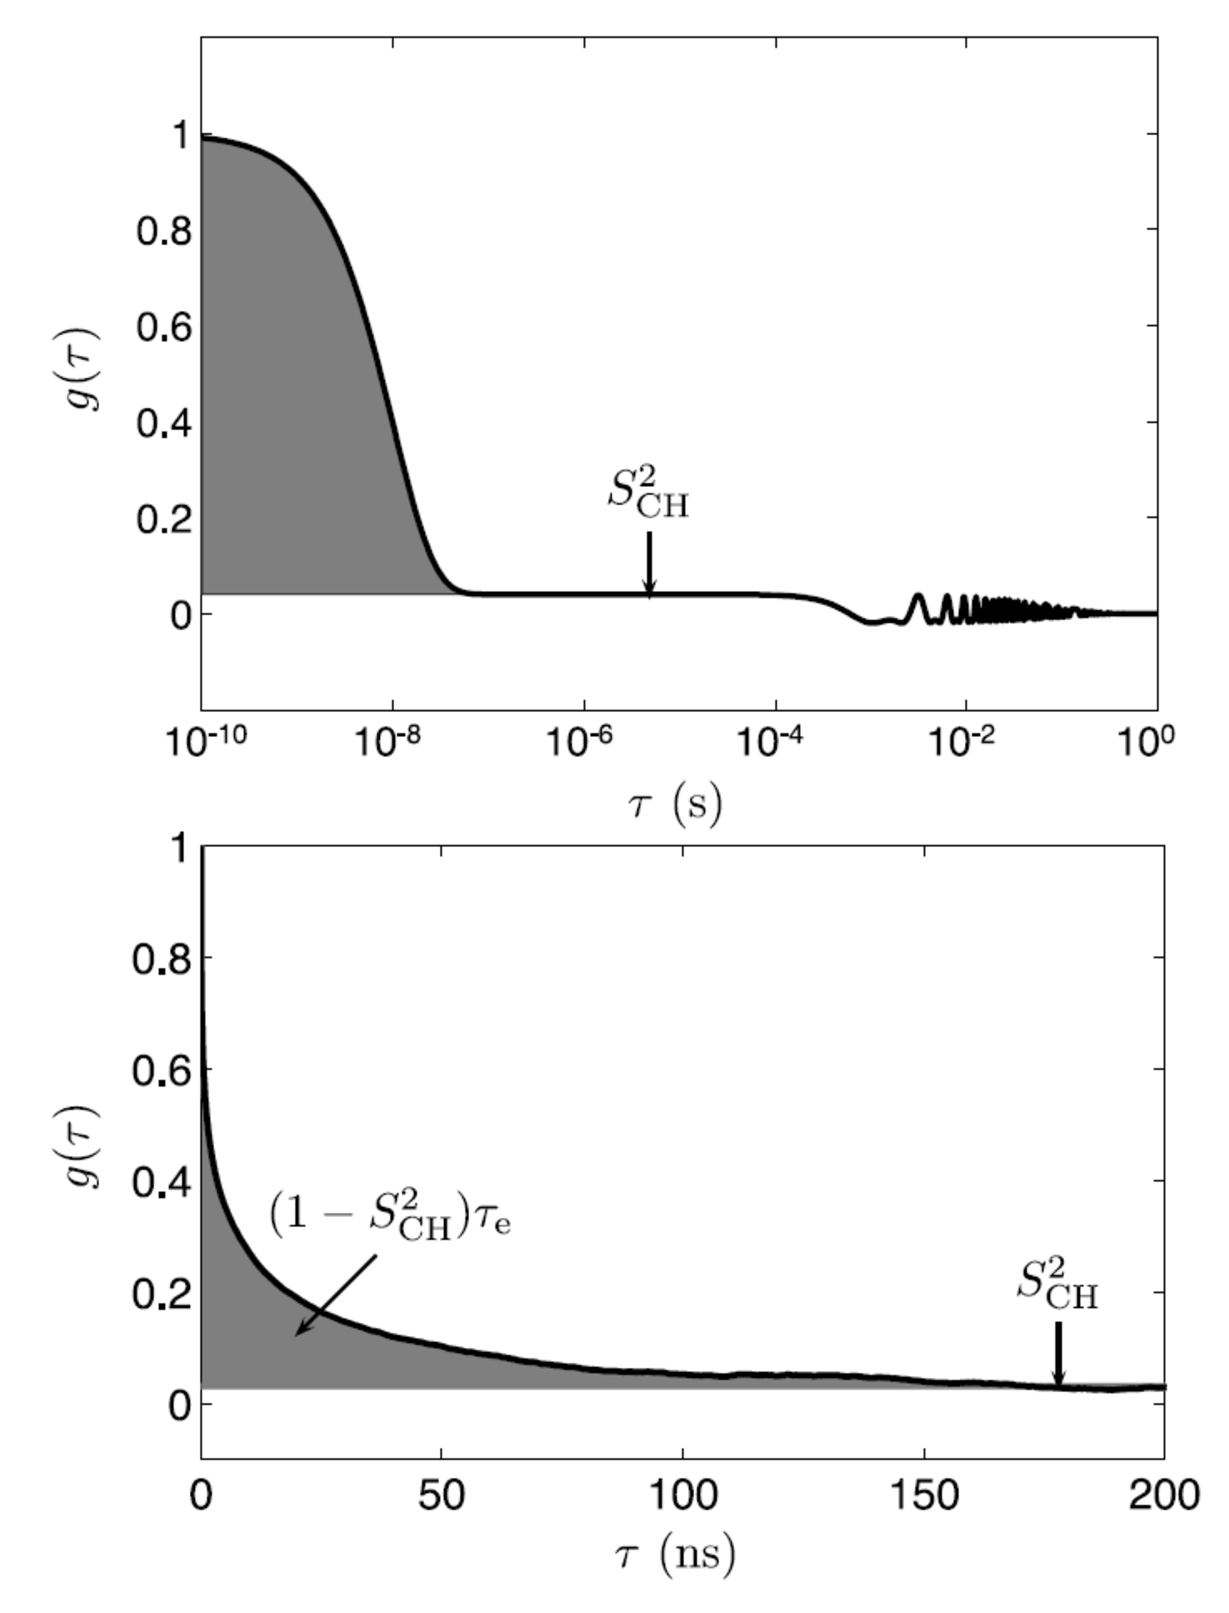
\includegraphics[width=8.6cm]{../Fig/correlationF.eps}
\newline
  \caption{\label{correlationF}
    (Top) Illustration of the auto-correlation function $g(\tau)$ and effective
    correlation time $\tau_e$ for a $^{13}$C-H bond in a lipid bilayer in MAS experiment (x--axis with logarithmic scale).
    Plateau after fast relaxation processes $g(\tau)_f$ is shown between roughly 10$^{-7}$s and 10$^{-4}$s.
    After this timescale the slow relaxation processes $g(\tau)_s$ and oscillation due to MAS~\cite{nowacka10} are shown.
    (Bottom) $g(\tau)$ for g$_1$ segment having the slowest relaxation in POPC bilayer simulated with the Berger based model,
    illustrating the decay towards $S^2_{{\rm CH}}$ (x--axis with linear scale). 
    This represents the $g(\tau)_f$ in Eq.~\ref{corrF} and decrease to the plateau in the top figure.
    The effective correlation time $\tau_e$ is equal to the area in gray scaled by $(1-S^2_{{\rm CH}})^{-1}$.
    Reprinted with permission from Ref.~\cite{ferreira15}. Copyright 2015 AIP Publishing LLC.
  } 
\end{figure}


The $g_{\rm{f}}(\tau)$ decays to the plateau having value of $S_{{\rm CH}}^2$ within few hundred nanoseconds 
in liquid crystalline lipid bilayers with planar symmetry~\cite{ferreira15}, as illustrated in Fig~\ref{correlationF}. 
The order parameters from $^2$H NMR and $^{13}$C NMR experiments are measured from this plateau~\cite{ferreira15},
thus the rotational correlation function describes the average time needed to sample all conformations for 
a single molecule within the bilayer plane. The effective correlation time~\cite{Lipari82}
\begin{equation}\label{effCTdef}
\tau_{e}:=\int_0^{\infty} \frac{g_{\rm{f}}(\tau)-S_{\rm{CH}}^2}{1-S_{\rm{CH}}^2} \mathrm{d}\tau
\end{equation} 
gives intuitive measure for this time; larger $\tau_e$ means longer time required for the conformational sampling.
With this definition the area between the correlation function and its pleateau becomes $(1-S_{\rm{CH}}^2)\tau_{e}$, 
as illustrated in Fig.~\ref{correlationF}.

\subsection{Detecting C--H bond dynamics experimentally}\label{dynamicsEXP}

The C--H bond dynamics in nanosecond timescales can be detected experimentally by measuring
the spin relaxation rates $R_1^C$ from $^{13}$C NMR and $R_1^D$ from $^2$H NMR. 
These are connected the molecular dynamics through the spectral density (Eq.~\ref{FT}) and equations \cite{harris86}
\begin{equation}\label{R1C}
R_{1}^{C}=\frac{D_{\rm{max}}^2N_{\rm{H}}}{20}\bigg[j(\omega_{\rm{H}}-\omega_{\rm{C}})+3j(\omega_{\rm{C}})+6j(\omega_{\rm{C}}+\omega_{\rm{H}})\bigg]
\end{equation}
and
\begin{equation}\label{R1D}
R_{1}^{D}=\frac{12\pi^2}{40}\bigg(\frac{e^2qQ}{h}\bigg)^2\bigg[j(\omega_{\rm{D}})+4j(2\omega_{\rm{D}})\bigg],
\end{equation}
where $\omega_{\rm{C}}$, $\omega_{\rm{H}}$ and $\omega_{\rm{D}}$ are the Larmor frequencies for $^{13}$C, $^1$H and $^2$H, respectively, 
$N_{\rm{H}}$ is the number of bound protons, $\frac{D_{\rm{max}}}{2\pi}\approx$22 kHz as in section~\ref{CopSECTION} and
$\frac{e^2qQ}{h}$=170kHz as in section~\ref{DopSECTION}.

As seen from Eqs.~\ref{R1C} and~\ref{R1D}, the numerical values of $R_1^{C}$ and $R_1^{D}$ depend on 
spectral density values at the Larmor frequencies $\omega_C$, $\omega_H$ and $\omega_D$.
On the other hand, the spectral density value for a given frequency $\omega$ 
depends on the relative amount of relaxation processes with timescales close to $\omega^{-1}$.
The Larmor frequencies depend on the spectrometer magnetic field strength and typical
timescales for $\omega^{-1}$ are $\sim$1-20ns in $^{13}$C NMR and $^2$H NMR experiments.
Thus, the $R_1^{C}$ and $R_1^{D}$ values measured with standard spectrometer with fixed external
field stregth gives a measure of relative amount of relaxation processes with the timescales $\sim$1-20ns.
Further, the measured changes gives only the change of the relative amount of dynamical processes with
the timescale detected, not the changes in sampling rate. For further discussion and demonstrations see e.g.~\cite{ferreira15}.

For more comprehensive dynamical picture the spin relaxation parameters are 
measured with different magnetic field strengths by using the field cycling NMR~\cite{roberts04a,roberts04b,roberts09,sivanandam09}
or several spectrometers with different magnetic field strengths, as recently reviewed by Leftin and brown~\cite{leftin11}.
Also the model free approach to measure the effective correlation time (Eq.~\ref{effCTdef}) was recently
introduced~\cite{ferreira15}. The method is based on the combination of experimental order parameter $S_{{\rm CH}}$,
spin-lattice relaxation rates $R_1^C$ and the transverse magnetization under a spin lock pulse $R_{1\rho}^{\rm{plateau}}$ 
measured with appropriate nutation frequency, given through equation

\begin{equation}\label{ECT}
\tau_{\rm{e}}\approx\frac{5R_{1\rho}^{\rm{plateau}}-3.82R_1^C}{D_{\rm{max}}^2N_{\rm{H}}(1-S_{\rm{CH}}^2)}.
\end{equation} 


\subsection{Analyzing C--H bond dynamics from simulations}


Since all the atom coordinates as a function of time are available from molecular dynamics simulations trajectory,
the auto--correlation function for each C--H bond can be calculated directly from the definition in Eq.~\ref{gt}.
The hydrogen positions can be generated post-simulationally based on heavy atoms 
positions and the known hydrocarbon geometries for united atom simulations without explicit hydrogens 
by creating a trajectory with added hydrogens~\cite{lindahl01,wohlert06a,ollila07a,ferreira15}. 
The ensemble average is taken over all the time intervals and molecules 
in present in simulation. Since the amount of data decreases for time intervals approaching the simulation total length,
only interval lengths less than half of the total simulation time are typically used; for more details see~\cite{gromacsMANUAL}.

To calculate the experimentally measurable spin lattice relaxation times from Eqs. \ref{R1C} and \ref{R1D}, 
the spectral density must be first calculated from auto-correlation function using Eq.~\ref{FT}. 
Usually sum of 4 or more exponentials are fitted to the calculated auto--correlation function and then 
analytical Fourier transform is used to calculate the spectral 
density~\cite{pastor88,venable93,pastor02,eldho03,ollila07a,ferreira15},
however some authors have also used streched exponential exponential functions~\cite{lindahl01,wohlert06a}.
The chosen functional form should not affect the spin relaxation rate values as long as the fit is good, however 
the correct form to describe the real relaxation process can be debated~\cite{leftin11,wohlert06a,edholm08,klauda08a,klauda08c}. 
Single exponential function is not enought to describe relaxation observed in simulations while 4 gives a reasonable 
fit~\cite{eldho03} which is not surprising since more than one relaxation timescales are expected to be present in bilayer
lipids~\cite{pastor88,venable93,pastor02,leftin11}. The $R_{1}^{C}$ and $R_{1}^{D}$ values are straighforward to
calculate from Eqs. \ref{R1C} and \ref{R1D} with different Larmor frequencies or as a function of external
field by using the analytical spectral density function with fitted parameters.

The effective correlation time $\tau_e$ can be calculated directly from the integrated area below the correlation 
function, see Fig.~\ref{correlationF} or by using the exponential sum fitted to the correlation function as  
in Eq. 30 of Ref.~\cite{ferreira15}. The $R_{1\rho}$, used to determine effective correlation time experimentally 
in Eq. \ref{effCTdef} cannot be calculated from simulations directly since its value may depend
also on the slow relaxation dynamics ($g_s(t)$ in Eq.~\ref{corrF}) which is not present in simulations \cite{ferreira15}.
The same applies to the calculation of NOESY relaxations rates for which the decay time of 170~ns was assumed for the
$g_s(t)$~\cite{feller99}, while 4.2~ms was measured by Ferreira et al.~\cite{ferreira15}.



\subsection{Comparing C--H bond dynamics between simulations and NMR experiments}

\begin{figure}[]
%  \centering
  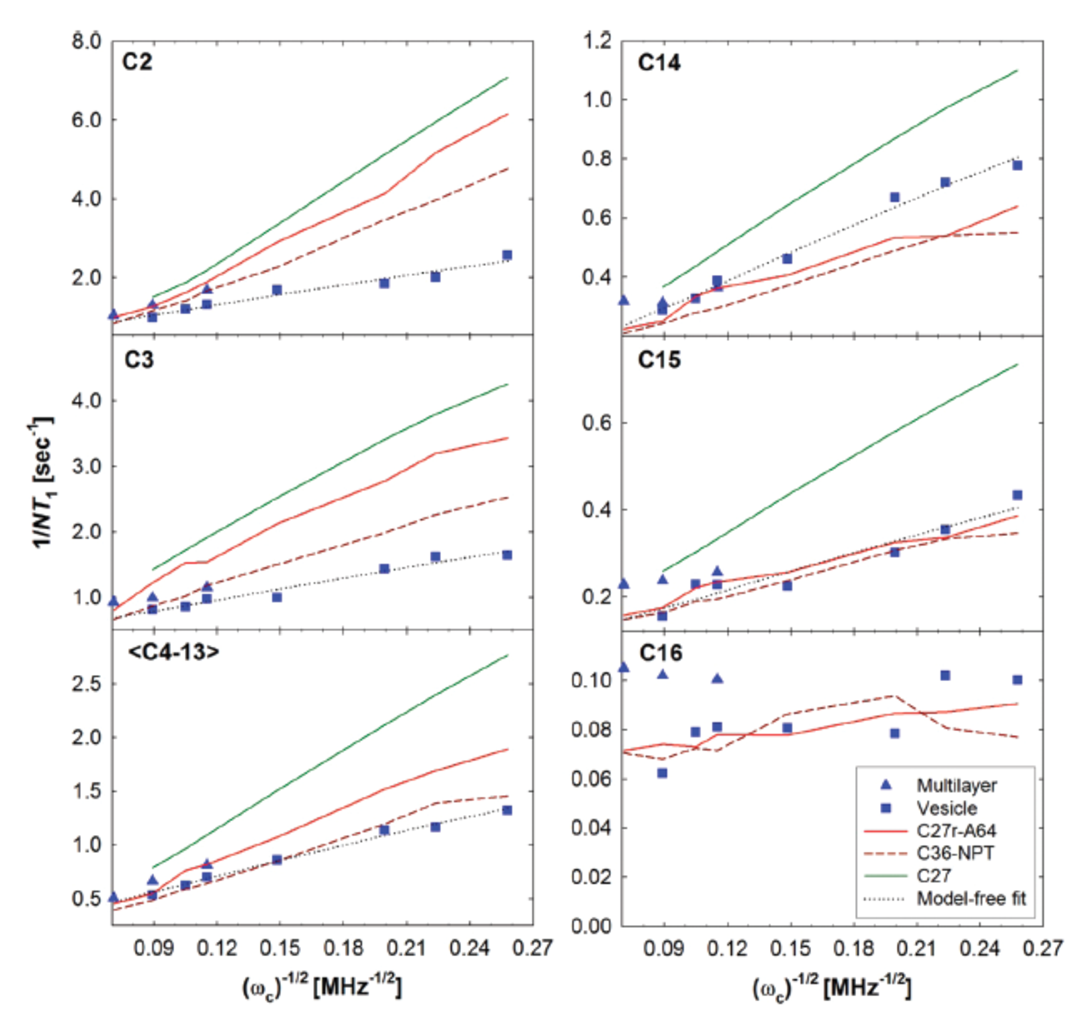
\includegraphics[width=8.6cm]{../Fig/RdisperisonCHARMM.eps}
\newline
  \caption{\label{RdispersionCHARMM}
    Comparison of $R_1^{C}$ dependence on magnetic field between experiments~\cite{brown83,klauda08a} and different CHARMM simulations~\cite{klauda10} 
    for acyl chain carbons (DPPC bilayer in 323K).
    Experiments as points; MD simulations as solid and dashed lines; and a model-free fit to the vesicle data as dotted lines. 
    Reprinted with permission from Klauda et al. J. Phys. Chem. B, {\bf 2010}, 114, 7830-7843. Copyright 2010 American Chemical Society.
     } 
\end{figure}
\begin{figure}[]
%  \centering
  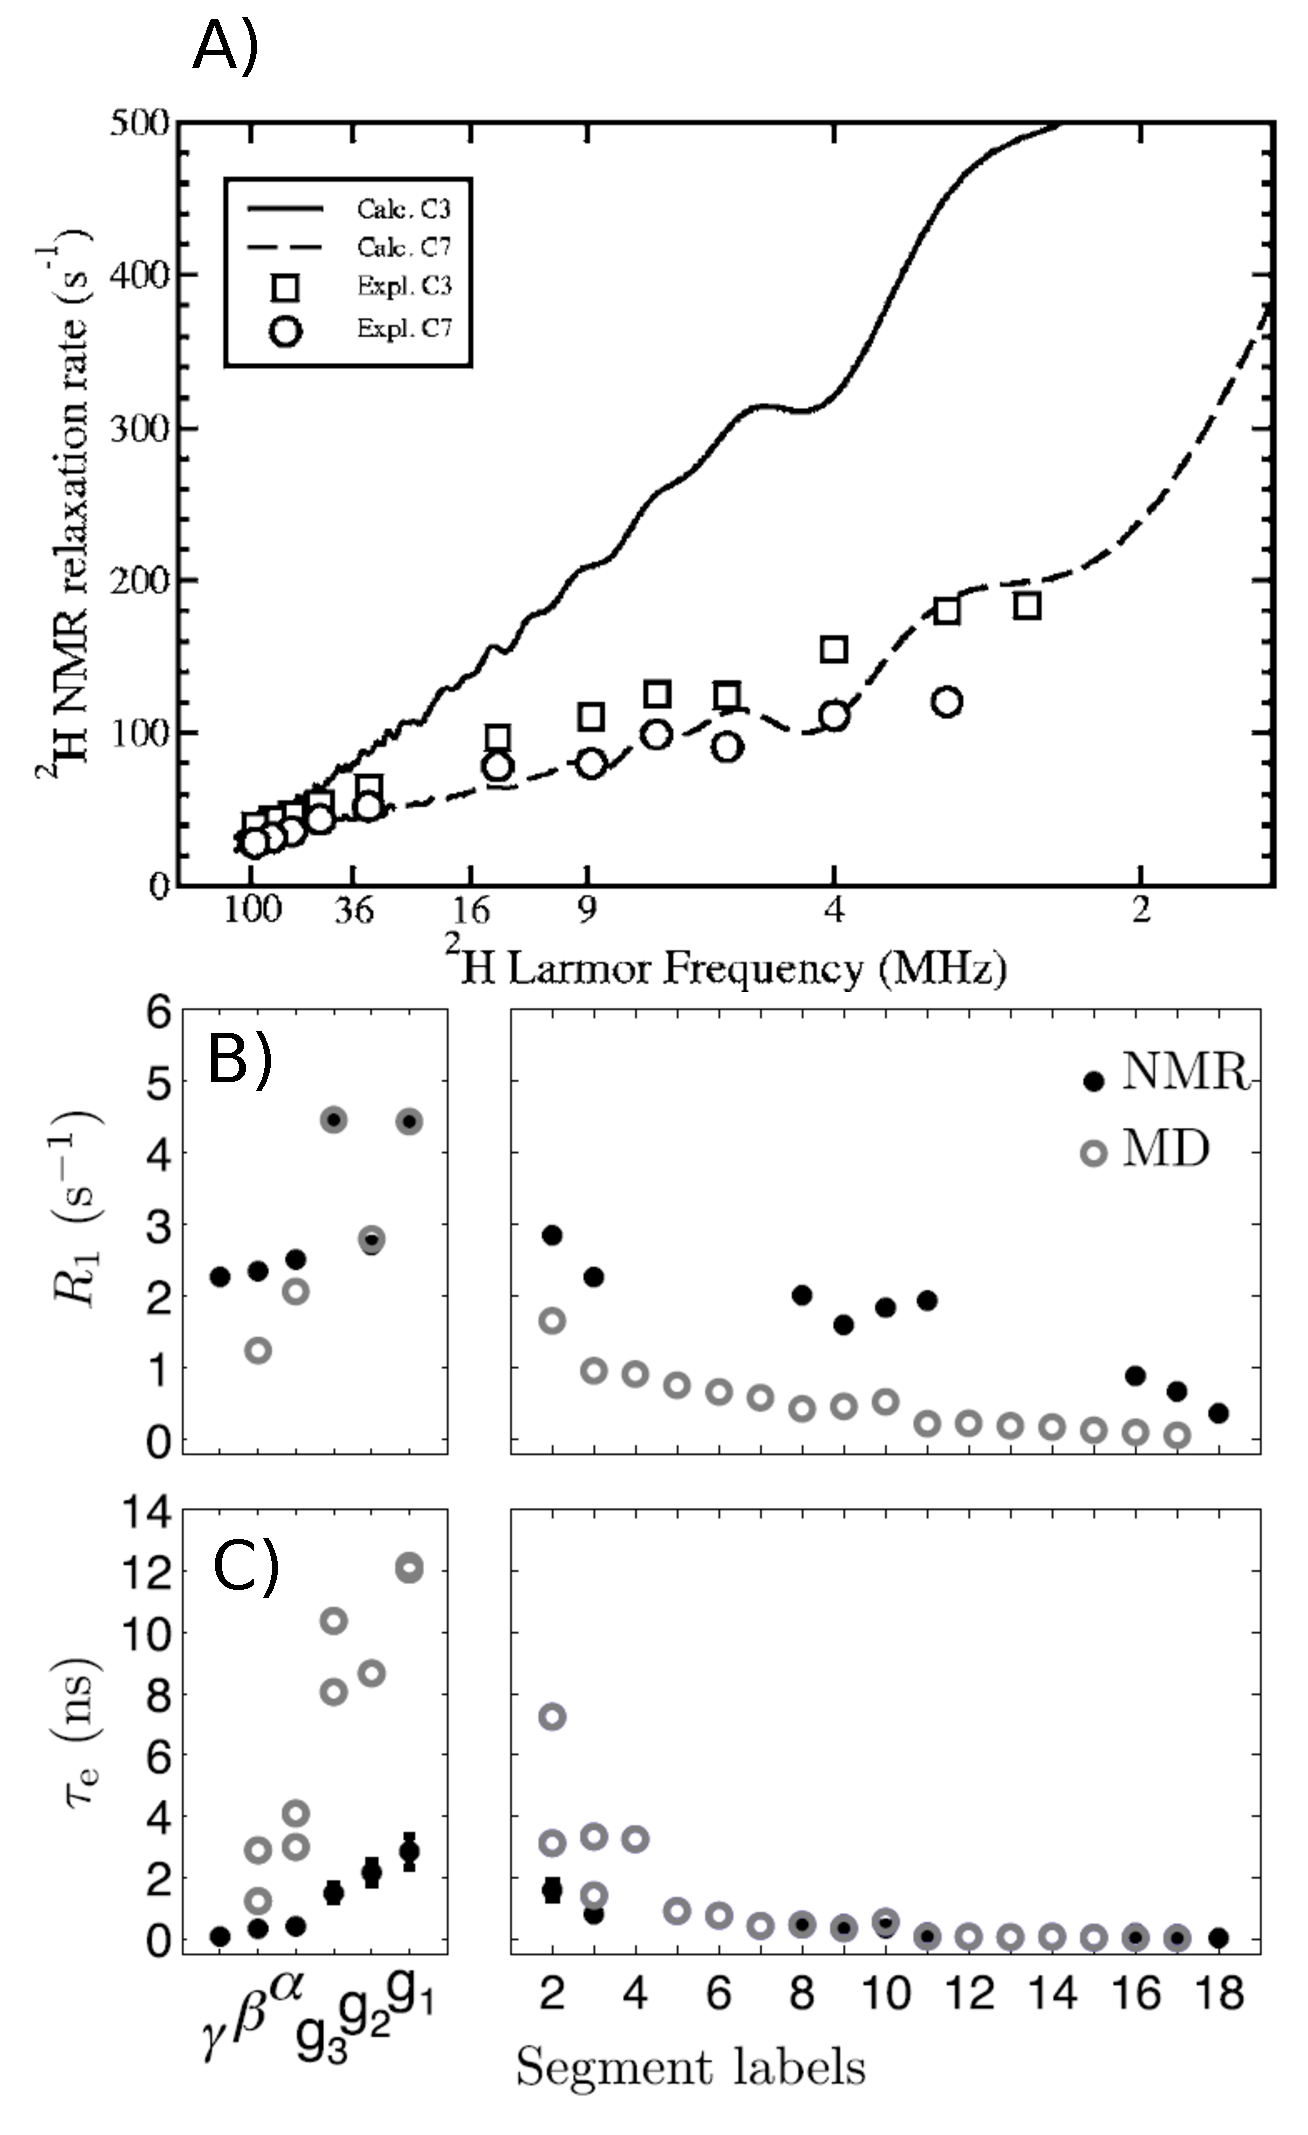
\includegraphics[width=8.6cm]{../Fig/RandEFFCT.eps}
\newline
  \caption{\label{RandEFFCT}
    Comparisons between Berger based models and experimental spin relaxation rates:
    A) $R_1^{D}$ dependence on magnetic field for acyl chain carbons (DMPC bilayer at 300K)~\cite{wohlert06a}.
    Reprinted with permission from Ref.~\cite{wohlert06a}. Copyright 2006 AIP Publishing LLC.
    B) $R_1^{C}$ measured with field strength correspondin to the Larmor frequency of 125 MHz for $^{13}$C (POPC bilayer at 298K) and
    C) effective correlation times $\tau_e$ (POPC bilayer at 298K). 
    Reprinted with permission from Ref.~\cite{ferreira15}. Copyright 2015 AIP Publishing LLC.
  } 
\end{figure}

Spin relaxation rates $R_1^{C}$ and $R_1^{D}$ with one~\cite{feller02,eldho03,ollila07a,klauda08b,ferreira15} 
or more ~\cite{pastor88,lindahl01,pastor02,klauda08a,klauda08b,wohlert06a,klauda12} external magnetic field 
strengths have been compared between experiments and simulations mainly for CHARMM (Fig. \ref{RdispersionCHARMM}) 
and Berger based models (Fig. \ref{RandEFFCT}). The comparison with several
magnetic field strengths shows good a agreement with large larmor frequencies 
for both CHARMM and Berger based models in Figs.~\ref{RdispersionCHARMM} and~\ref{RandEFFCT} A), respectively.
With increasing larmor frequencies both models show a good agreement deep in the acyl chain region
while closer to the interfacial region motional modes corresponding lower Larmor frequencies seems to overpresented
in both models. Since lower Larmor frequencies correspond longer correlation times, this may
indicate too slow dynamics close to the interfacial region. 

This is in line with the comparison between experimental and simulated effective correlation times for Berger
based POPC model, shown in Fig.~\ref{RandEFFCT} C); the effective correlation times for acyl chain region agrees 
with experiments while closer to the interfacial region the correlation times are too large in simulations. 
The discrepancies for $R_1^{C}$ between experiments and simulations for acyl chain region shown in Fig.~\ref{RandEFFCT} B)
indicate, however, that different dynamical processes are not correctly balanced in simulations despite of good
agreement for $\tau_e$.  On the other hand, spin relaxation rates for polyunsaturated acyl chains
with large Larmor frequenciens give reasonable values for both, CHARMM~\cite{eldho03,klauda12} and Berger 
based~\cite{ollila07a} models.




\subsection{Interplay between simulations and NMR spin lattice relaxation times: Validation and interpretation of dynamics}

Most importantly, the fairly good agreement for spin relaxation rates and effective correlation times between 
simulations and experiments in acyl chain region indicates that the lipid rotational dynamics has the 
correct order of magnitude in simulations. Consequently, the rapid acyl chain fluctuations observed in 
simulations can be considered as realistic which further supports the advantage of simulation videos as an
intutitive lipid bilayer picture compared to the traditional static pictures. While the molecular sampling rates 
seems to be underestimated closer to the interface, also the sampled structures are not excatly correct
in simulations \cite{botan15}, thus the sampling rates in simulations are mainly interesting only for people 
improving the models. 

As discussed in Section \ref{dynamicsEXP} and for example in Ref. \cite{ferreira15},
single measured spin relaxation rate values or changes are not straightforwardly connected
to the molecular dynamics. MD simulations can significantly ease this connection if the
experimental spin relaxation rates or their differences can be reproduced~\cite{feller02,eldho03,nowacka13}.
This has been especially useful in the studies of polyunsaturated acyl chain dynamics which concluded --
by combining the simulation and NMR relaxation data -- that the double bonds speed up the chain dynamics
due to flexible dihedrals next to the double bonds~\cite{feller02,eldho03,gawrisch03,stillwell03}.

The successfull interpretation of relaxation time measurements with MD is significantly less laborious
than careful studies with different temperatures and magnetic field strengths, recently reviewed by 
Leftin and Brown~\cite{leftin11}. On the other hand, the interpretation is also eased by  
the recently introduced effective correlation time experiments~\cite{ferreira15}.
For example, careful compilation of several experimental data sets with different
temperatures and magnetic fields was needed to conclude that the lipids has slower dynamics in
interfacial region than in the acyl chains region~\cite{leftin11}, while the same conclusion
is obvious from the measured effective correlation times in Fig.~\ref{RandEFFCT} \cite{ferreira15}.
The same is seen also in the MD simulations, however, the simulation model quality is not
yet on the level to be used alone for interpretataion for interfacial region.

Lipid bilayer rotational modes have been often interpreted with the 
wobble in the cone model~\cite{pastor88,pastor02,klauda08a,klauda08c,sivanandam09} suggesting
that the whole lipid molecule is wobbling as a cone and that all lipid segments share the same time scale for 
this motion. Further timescales for segmental dynamics then arises from the dynamics inside the cone. 
The auto--correlation functions predicted by the model are successfully fitted to the simulation and 
experimental data~\cite{pastor88,pastor02,klauda08a,klauda08c,sivanandam09}, however,
fits with similar or better quality would be probably possible also with other type of models as well.
In addition, significant changes of structure and dynamics experienced in the acyl chain region may not 
hinge on the headgroup~\cite{ferreiraTHESIS,botan15} indicating weak coupling 
between these segments, in line with one plausible interpretation for recent field cycling 
experiments~\cite{roberts09}. Also the role of membrane undulations in the low frequency 
relaxation data is still under discussion~\cite{leftin11,edholm08,klauda08a,klauda08c}.
Thus, the wobbling in the cone is not yet fully proven to be the correct description for lipid
rotational dynamics. Lipid models with realistic rotational dynamics for all segments 
with all timescales could elucidate this issue significantly.





%\newpage


\section{Form factors from scattering and simulations}

%\noindent {\bf For this section I would be more than happy for some help} \\[0.1cm]

\subsection{Form factor measured with X-ray or Neutron scattering}

Small-angle X-ray or neutron scattering (SAXS/SANS) experiments can be used to
probe the overall structure of the lipid bilayer, in particular scattering length density profiles along normal axis.
%As far as I understand these are not directly measured: membrane thickness, area per lipid or lipid chain length. 
The measured scattering intensity can be written as 
$I(q)\sim|F(q)|^2S(q) / C_{{\rm LF}}$, where $F(q)$ is the bilayer form 
factor, $S(q)$ is the structure factor and $C_{{\rm LF}}$ the Lorentz correction ($C_{{\rm LF}} = q^2$ 
for free-floating lipid vesicles and $C_{{\rm LF}}=q$ for aligned bilayers). 
The structure factor characterizes the crystalline or quasicrystalline structure of bilayer 
stacks and the form factor describes the scattering length density distribution of the lipid bilayer 
itself along the bilayer normal. 

Here the main interest lies in the form factor since we focus on the lipid bilayer structure.
The scattering intensity can be measured from unilamellar vesicles (ULVs)~\cite{marquardt15}, 
oriented multilamellar bilayes (ORI)~\cite{Lyatskaya.2001,kucerka05a} and un-oriented multilamellar vesicles (MLVs)~\cite{Heftberger.2014}.
Information about the structure factor is needed to extract the 
form factor from the scattering intensity, except for positionally uncorrelated ULVs, where $S(q)=1$~\cite{marquardt15}. 
For multibilayers in the fluid phase the structure factor is given by the Caill\'{e} theory~\cite{Zhang.1994,Lyatskaya.2001}. 
For oriented samples the form factor is determined by scaling a 2D fit of the Caill\'{e} structure factor 
(for in-plane and out-of-plane scattering constributions) to the measured scattering intensity~\cite{Lyatskaya.2001,kucerka05a}.
For MLVs the form factor needs to be modeled in combination with the structure factor to fit the scattering intensity~\cite{Heftberger.2014}. This is achieved by using a specific real-space description of the bilayer structure (scattering length density profile). Note that different real-space model yield equivalent form factors. Thus, the form factors are not highly sensitive to the applied model.
Different technical issues must be carefully considered in all scattering experiments, in particular 
subtracting background scattering and, in the case of ORI and MLVs, fitting accuracy. The form factors measured 
from different geometries~\cite{kucerka05a,kucerka05b,kucerka07} and research groups are in good agreement
as demonstrated in Fig.~\ref{FFs}, indicating that the bilayer structure is similar in different preparations of the same lipid and that the technique is highly robust.
\begin{figure*}[]
	%  \centering
	\includegraphics[width=12.2cm]{../Fig/FFs.eps}
	\caption{\label{FFs}
		Comparison of reported X-ray (left panel) and neutron (right panel) form factors for POPC bilayers at 303K in different geometries
                measured by different groups: Heftberger et al. (2014)~\cite{Heftberger.2014}, Kucerka et al. (2011)~\cite{kucerka11} and Kucerka et al. (2005)~\cite{kucerka05b}.
                The error bars given for neutron data by Kucerka et al. (2011)~\cite{kucerka11} are the same size as the line width.
	} 
\end{figure*}

By following the notation from Ref. \cite{kucerka10}, the form factor is connected to the bilayer atom number density through the 
equation 
\begin{equation}\label{FF}
|F(q)|=|\int_{-D/2}^{D/2}(\sum_\alpha f_\alpha(q_z)n_\alpha(z) - \rho_s) \exp(i z q_z) {\rm d}z|,
\end{equation}
where $n_\alpha(z)$ is the atom $\alpha$ number density as a function of membrane normal coordinate $z$,
$f_\alpha(q_z)$ is the atom scattering length density,
$\rho_s$ is the solvent scattering length density and integral spans over the bilayer of thickness $D$.
The atom scattering length density $f_\alpha(q_z)$ depends on the type of scattering used since
X-ray photons interact with the sample's electron cloud, while neutron scatter off nuclei in a particular manner.
This leads also to distinct contrast for different parts of the membrane. X-rays, for example are most sensitive to the electron-rich 
phospholipid headgroups. Neutron experiments typically explore the contrast between hydrogen and deuterium~\cite{marquardt15},
e.g. SANS on protiated lipid bilayers suspended in 100\% D$_2$O probes mainly the membrane's hydrophobic thickness
and specifically deuterated lipids are used to study lipid structural details \cite{buldt78,buldt79}.
Also, e.g. $^{44}$Ca has been used to detect Calcium location in lipid bilayer \cite{herbette84}.
Consequently, highest-structural resolution can be achieved upon combining SAXS and SANS experiments~\cite{kucerka05a,kucerka08a}.

For symmetric lipid bilayers Eq.~\ref{FF} simplifies to the widely used form
\begin{equation}\label{FFsimpl}
|F(q)|=|\int_{-D/2}^{D/2}\Delta \rho_e(z) \cos(zq_z) {\rm d}z|,
\end{equation}
where $\Delta \rho_e(z)$ is the scattering length density difference between solvent and bilayer.

%\onecolumngrid
%\todo{Discussion about related issues can be found at:
%{\tt https://github.com/NMRLipids/NMRLipids\_V-Review/issues/1}}


%\todo{The discussion is going in at: 
%{\tt https://github.com/NMRLipids/NMRLipids\_V-Review/issues/2} 
%}
%\twocolumngrid

\subsection{Form factor calculation from simulations}
The atomic number densities $n_\alpha(z)$ are straighforward to calculate from simulations and
then substitute into Eq.~\ref{FF} to calculate the form factor. The atomic scattering 
length densities $f_\alpha(q_z)$ for neutrons are available in the literature~\cite{sears92}.
For x-ray scattering pointwise valence electron location at the atom positions is usually assumed 
and in this case the $f_\alpha(q_z)$ becomes the number of electrons per atom,
while also gaussian electron distribution around atom positions~\cite{benz05} or an analytical expression 
$f_\alpha(q_z)=\sum_{j=1}^4a_je^{-b_j(q/4\pi)^2}+c$ with parameters $a_j$, $b_j$ and $c$ taken from~\cite{cromer68}  
are assumed in some studies~\cite{benz05}, including the widely used SIMtoEXP software~\cite{kucerka10}.
The effect of these choices to the electron density profiles was discussed by Benz et al.~\cite{benz05}, 
however, it is not clear how strongly this would affect form factors calculated from simulations.
In most simulations the bilayer is symmetric, thus the simpler Eq.~\ref{FFsimpl} is used. 

The small bilayer patches used in simulations might depress bilayer undulation modes which are present in large 
scale experiments~\cite{braun11}. Braun et al. showed that undulations seen in large simulations do
not change the location of form factor minimas but depress the peak hights in the lobes~\cite{braun11}.
Since the undulations are expected to be present in the experiments, the potential discrepancies 
between simulations and experiments in the lobe heights may be explained by the lack of undulation 
motions in simulations. The undulation effects are also sometimes reduced from the experimentally 
reported form factors by scaling $q$ in x--axis, however, the scaling factor is very close to 1~\cite{kucerka05a}.

Simulations give the form factors on absolute scale while experiments obtain them only on a relative scale,
thus the experimental form factors from different sources has to be scaled for comparison~\cite{kucerka08a,kucerka10}.
For example, the SIMtoEXP program uses the scaling factor $k$ defined as 
\begin{equation}
k=\frac{\sum_{i=1}^N\frac{|F_s(q_i)||F_e(q_i)|}{(\Delta F_e(q_i))^2}}{\sum_{i=1}^N\frac{|F_e(q_i)|^2}{(\Delta F_e(q_i))^2}},
\end{equation} 
where $F_e(q)$ and $F_s(q)$ are experimental and simulated form factors, respectively, $\Delta F_e(q)$ is the uncertainty
of the experimental form factor and the summation goes over all $N$ data points~\cite{kucerka08a,kucerka10}.
%In many studies which compare the form factors between experiments and simulations, the details on the scaling
%factor used is not given~\cite{??}. 

%\onecolumngrid
%\todo{More discussion at: \\
%{\tt https://github.com/NMRLipids/NMRLipids\_V-Review/issues/3} \\
%and \\
%{\tt https://github.com/NMRLipids/NMRLipids\_V-Review/issues/4} 
%}
%\twocolumngrid

\subsection{Comparing form factors between simulations and experiments}

The comparison to experimental area per molecule values to validate the lipid density in simulations~\cite{tieleman97} has
been nowdays often replaced with more direct comparison~\cite{nagle00} using x-ray form 
factors~\cite{hogberg08,chiu09,klauda10,dickson12,jambeck12,lim12,klauda12,jambeck13,chowdhary13,lee14,maciejewski14,dickson14,tjornhammar14,madej15,kulig15b}.
In some studies the comparison is complemented with the comparison to the neutron scattering 
data with D$_2$O~\cite{dickson12,jambeck12,lee14,dickson14,tjornhammar14,madej15}.
In general the models produce form factors in good agreement with experiments for pure lipid bilayers, especially at small $q$ values indicating 
that the overall bilayer dimensions, like thickness, are reproduced reasonably well. However, the agreement gets often worse
toward higher $q$ 
values~\cite{chiu09,klauda10,klauda12,dickson12,lim12,jambeck12,chowdhary13,jambeck13,lee14,maciejewski14,dickson14,kulig15b,madej15}
(see Fig.~\ref{FFcomp}), indicating discrepancies in fine structural details such as, e.g. hydrocarbon chain packing or headgroup structure.
Typically, the comparison of experimental and simulated form factors is based on visual inspection while also quantitative measure
for simulated form factor quality has been suggested~\cite{kucerka10}. In some studies also Fourier transform coeffiecients are
compared~\cite{benz05}
\begin{figure*}[]
%  \centering
  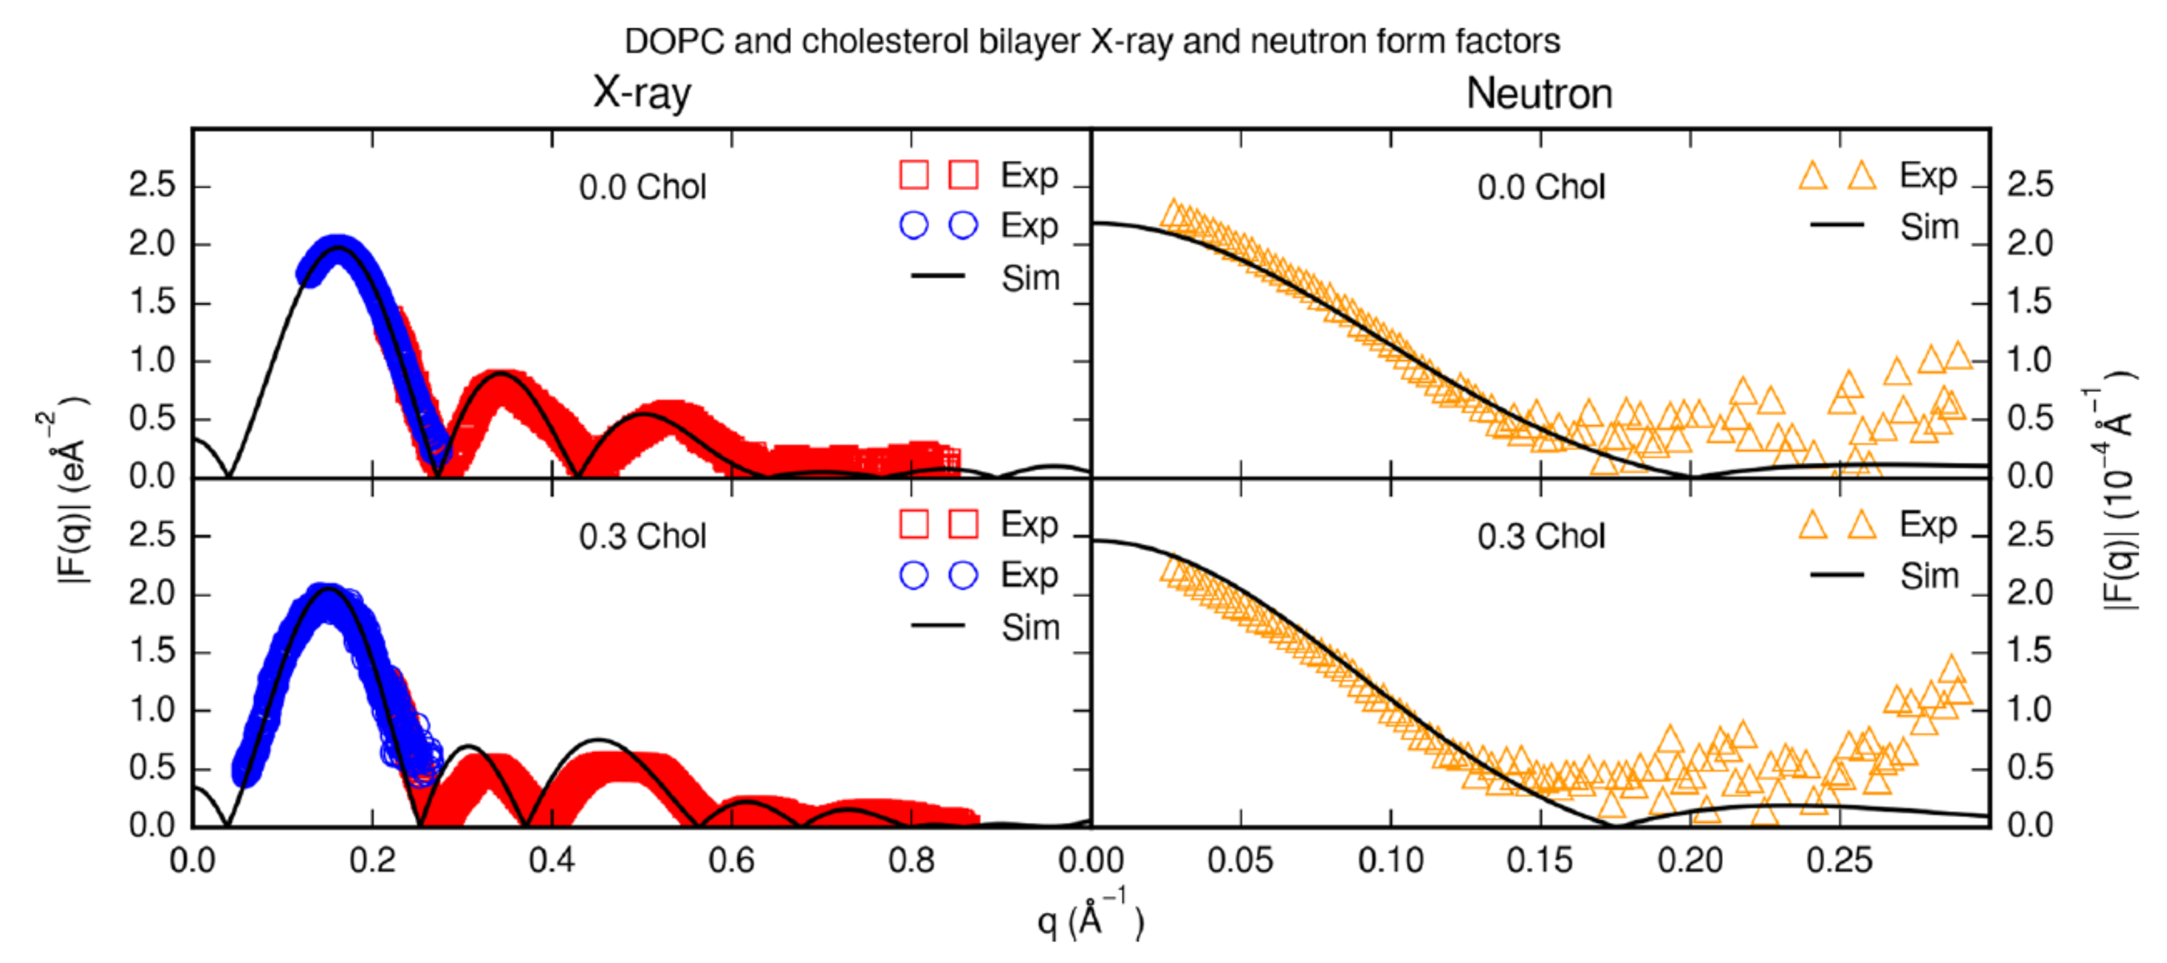
\includegraphics[width=12.2cm]{../Fig/FFcompMADEJ.eps}
\newline
  \caption{\label{FFcomp}
    Comparison of experimental~\cite{pan09,kucerka07b} and simulated (using Amber Lipid14 ~\cite{madej15}) X-ray and neutron form factors for pure DOPC bilayers and DOPC/cholesterol ($x_{chol} = 30$ mol\%) mixtures. Within experimental uncertainty, simulations argee well with neutron data. For X-ray data, simulations match well DOPC experimental data at low $q$, but are slightly off for the third lobe, indicating  some differences in the lipid bilayer fine structure. The DOPC/cholesterol mixture clearly shows disagreement between model and experiment for $q > 0.3$\AA$^{-1}$. Overall, the simulated form factor minima are shifted toward lower $q$, revealing an overestimated bilayer thickening effect of cholesterol. Reprinted with permission from Madej et al. {\bf 2015}, 119, 12424-12435. Copyright 2015 American Chemical Society.
  } 
\end{figure*}

Also changes in form factor due to temperature~\cite{jambeck12,zhuang14}, cholesterol concentration~\cite{jambeck13,madej15} 
and acyl chain polyunsaturation~\cite{eldho03,klauda12} have been compared between simulations and 
experiments~\cite{eldho03,kucerka05a,pan08,hodzic08,kucerka08a,pan09,khelasvili10,kucerka11}.
Simulation generally reproduce the decreased thickness and increased area with increasing temperature~\cite{jambeck12,zhuang14} and 
polyunsaturation level~\cite{eldho03,klauda12}, 
as well as increased thickness and decreased area with increasing cholesterol concentration~\cite{jambeck13,madej15}.
However, the temperature dependence is underestimated for some systems~\cite{jambeck12,zhuang14} while cholesterol
effect is overestimated~\cite{jambeck13,madej15}, in good agreement with the comparisons to the NMR order parameter 
data~\cite{zhuang14,madej15}, as discussed in Section~\ref{OPcompSECTION}. Example of form factor comparison 
between experiments and simulations is shown in Fig. \ref{FFcomp}.
Atomistic resolution simulations have not been able to reproduce the special cholestrol orientation, lying flat in
the middle of polyunsaturated lipid bilayer, as observed with neutron scattering~\cite{harroun08,marrink08,kucerka10b}.

In conclusion, all the state of the art simulation models gives form factors close to experimental
data in various conditions indicating reasonable agreement for average bilayer dimensions. Also the qualitative changes are reproduced, however, 
discrepancies prevail for quantitative details of bilayer structure and changes with temperature and admixture of other lipids such as cholesterol.


\subsection{Interplay between simulations and scattering experiments: Validation and interpretation}
The scattering form factor gives accurate information about lipid
bilayer structure but a model for atom number densities, $n_\alpha(z)$ in Eq.~\ref{FF}, is needed to 
resolve the structure, analogously to the NMR order parameters. Further, several atom density
profiles can reproduce essentially the same form factor \cite{kucerka08a}, thus also independent information is needed to 
confirm the structures suggested by the models, also analogously to the NMR order parameters. 
As already discussed in Section \ref{OPdefinition}, significant advantage of MD model is that the same model 
can be straightforwardly compared to both, NMR and scattering data.

Several models, reviewed by Heberle et al.~\cite{heberle12}, are developed to give structural interpretation 
for the form factor data \cite{fogarty15},  while also MD simulations are 
used~\cite{sachs03,klauda06,kucerka08a,kucerka08b,braun13}. In these studies the area per molecule 
is often fixed to a value minimizing the differences between experimental and simulated form 
factors~\cite{sachs03,klauda06,kucerka08a,kucerka08b,braun13}. Depending on the model used, this
area per molecule may be close to \cite{braun13} or deviate 
significantly \cite{sachs03,klauda06,kucerka08a,kucerka08b} from the value predicted 
by the model in constant pressure simulations. However, with optimized area per molecule all models give
form factors close to the experiments, despite of the bilayer tension generated in some models.
On the other hand, comparisons between MD simulations and SDP model suggest small but measurable 
structural differences~\cite{kucerka08a,braun13}. The form factor from SDP model agrees better
with experiments and stuctural parameters indicate differences especially in the 
glycerol backbone and the headgroup regions~\cite{kucerka08a,braun13}, 
in agreement with comparison between simulations and NMR order parameters~\cite{botan15}, 
as discussed in section~\ref{OPinterplay}.

More accurate understanding on the quality of interactions in lipid mixtures, e.g. with cholesterol is needed 
to use the simulations to interpret the scattering data from multicomponent systems~\cite{heftberger15} or the special
cholesterol orientation in polyunsaturated bilayers~\cite{harroun08,marrink08,kucerka10b}.

%\onecolumngrid
%\todo{The more detailed discussion can be found at: \\
%{\tt https://github.com/NMRLipids/NMRLipids\_V-Review/issues/5}}
%\twocolumngrid


\section{Conclusions}

The comparisons of lipid bilayer C--H bond order parameters, spin relaxation rates and
scattering form factors between MD simulations and experiments for the validation and 
interpretation of the sampled atomistic resolution structures are reviewed.
The segmental order parameters and spin relaxation rates, measured with NMR, 
are related to the sampled structure and dynamics of individual molecules, while the
scattering form factor is related to the average structure of the whole bilayer.
NMR and scattering experiments are both highly robust and directly comparable to simulations, 
thus the sampled lipid and bilayer structures in MD model can be realistic only if these experimental 
quantities are reproduced with sufficient accuracy. Such an MD simulation model 
would be an ultimate tool to jointly interpretate the NMR and scattering data.
Further, such a model reproducing numerous independent experimental observables
could be  considered as the realistic atomistic resolution representation with high
probability. 

The current MD simulation models are yet not quite cabable of achieving this goal.
However, with current computational resources and available experimental
data the community has a fair change to create truly realistic atomistic resolution 
representations of lipid bilayers. More specifically: \\
- Atomistic resolution MD simulations give realistic structures and rotational dynamics
with correct order of magnitude for saturated and unsaturated acyl chains for PC lipid 
bilayers in full hydration close to 300K (or 323K for DPPC). Thus, the videos given
by simulations can be considered as a realistic intuitive picture about the acyl chain region.\\
- Qualitative changes in the acyl chain region with temperature, dehydration and cholesterol are
correctly described, however, in many cases the quality of detailed atomistic resolution changes are not clear. \\
- Current MD simulations are not yet accurate enough to resolve the atomistic resolution 
properties of glycerol backbone and choline regions, however, some structural changes can be 
correctly reproduced. Extreme care must be taken when simulation results are used to study, 
e.g. lipid--ion or lipid--cholesterol interactions on this region. \\

Similar conclusions are often made from the comparisons between simulations and two complementary 
experimental techniques, NMR and scattering, the first one related to the average properties
of individual molecules and the latter to the average bilayer properties. 
In wider perspective it seems that atomistic MD simulations, NMR spectroscopy and scattering all gives
complementary and coherent information on atomistic resolution biomolecular structure and dynamics. 
This indicates that the combination of these techniques has a realistic potential to generate atomistic 
resolution dynamical models of biomolecules in biologically relevant fluid state. However, the
main barrier that currently needs to be overcome seems to be the quality of the interactions described in MD models.

The demand for atomistically accurate MD models will most likely increase in near future with increasing
amount of accurate experimental data due the development in NMR methodology  
for lipids \cite{ferreira13,leftin13,leftin14,ferreira15,pham15} and proteins \cite{hansen15}, 
as well as due to the availability, e.g. wide-angle x-ray scattering of lipid bilayers, probing short-range positional 
correlations between hydrocarbons~\cite{spaar.2003}. 

The inaccuracies of simulation models in the interfacial region may also hamper the simulation 
studies of different biochemical systems. For example, proteins approaching
PC lipid bilayer in physiological NaCl concentration may encounter an effectively positively charged 
lipid bilayer due to artificial Na$^+$ binding with incorrect choline structure. In addition,
the protein might sample incorrect states already in the bulk water~\cite{best11,beauchamp12,rauscher15}.
From such a simulation it is difficult to filter results arising purely from simulation artefacts.
Thus, improvements of force fields underlying MD simulations are strongly encouraged.



% If you have acknowledgments, this puts in the proper section head.
\section*{acknowledgements}
This work is done by the NMRlipids Open Collaboration project running at \url{nmrlipids.blogspot.fi}
and \url{https://github.com/NMRLipids}. 
We acknowledge Nobert ku{\v c}erka and Frederick Heberle for sharing data for Fig.~\ref{FFs}. 
Markus Miettinen and Peter Heftberger are acknowleded for useful comments.
O.H.S.O. acknowledges financial support by the Emil Aaltonen Foundation.
G.P. acknowledges financial support by the Austrian Science Funds (FWF), grant no.~P24459.


\section*{References}
\bibliography{refs.bib}


\end{document}
